\documentclass[conference]{IEEEtran}
\usepackage[utf8]{inputenc}
\usepackage{textcomp}
\usepackage[spanish]{babel}
\usepackage{amsmath}
\usepackage{amsfonts}
\usepackage{amssymb}

\usepackage{graphicx}
%\usepackage{xcolor}
% Dependencies for Excel2Latex
\usepackage[table]{xcolor}
\usepackage{booktabs}
\usepackage{multirow}
% Dependencies for Excel2Latex
\usepackage{listings}
%Dependencies for [1.]
\usepackage{enumerate}
%Dependencies for [1.]
\usepackage{tikz}
\usepackage{float}
\usepackage{karnaugh-map}
\usepackage{adjustbox}
\usepackage[left=1cm,right=1cm,top=1cm,bottom=1cm]{geometry}
%Habilita bookmarks en PDF
\newcommand\MYhyperrefoptions{bookmarks=true,bookmarksnumbered=true,
pdfpagemode={UseOutlines},plainpages=false,pdfpagelabels=true,
colorlinks=true,linkcolor={black},citecolor={black},
urlcolor={black}}
\usepackage[\MYhyperrefoptions]{hyperref}
%Titulo del documento
\title{Proyecto Final: Aplicación para pizzeria}

\makeatletter
\newcommand{\linebreakand}{%
  \end{@IEEEauthorhalign}
  \hfill\mbox{}\par
  \mbox{}\hfill\begin{@IEEEauthorhalign} \hfill
}
\makeatother

\renewcommand\thesection{\arabic{section}}
\renewcommand\thesubsection{\thesection.\arabic{subsection}}
\renewcommand\thesubsubsection{\thesubsection.\arabic{subsubsection}}

\author{
	\IEEEauthorblockN{\hfill Kenneth Abarca Coronado \hfill}
	\IEEEauthorblockA{\textit{Estudiante Ing. en Sistemas de Computación}\\ 
	\textit{Universidad Fidélitas}\\
	San José, Costa Rica \\
	\href{mailto:Kabarca20607@ufide.ac.cr}{Kabarca20607@ufide.ac.cr}}
\and
	\IEEEauthorblockN{\hfill Jonathan Chavarria Peña \hfill}
	\IEEEauthorblockA{\textit{Estudiante Ing. en Sist. Computación}\\ 
	\textit{Universidad Fidélitas}\\
	San José, Costa Rica \\
	\href{mailto:jonach1998@gmail.com}{jonach1998@gmail.com}}
\and
	\IEEEauthorblockN{\hfill Erick Corrales Montero\hfill}
	\IEEEauthorblockA{\textit{Estudiante Ing. en Sist. Computación}\\
	\textit{Universidad Fidélitas}\\
	San José, Costa Rica \\
	\href{mailto:ecorrales00712@ufide.ac.cr}{ecorrales00712@ufide.ac.cr}}
\linebreakand % <------------- \and with a line-break
	\IEEEauthorblockN{\hfill Marco Fonseca Solorzano \hfill} 
	\IEEEauthorblockA{\textit{Estudiante Ing. en Sist. Computación}\\
	\textit{Universidad Fidélitas}\\
	San José, Costa Rica \\
	\href{mailto:marcosfin0232@gmail.com}{marcosfin0232@gmail.com}}
\and
	\IEEEauthorblockN{\hfill Keren Jimenez Fernandez \hfill} 
	\IEEEauthorblockA{\textit{Estudiante Ing. en Sist. Computación}\\
	\textit{Universidad Fidélitas}\\
	San José, Costa Rica \\
	\href{mailto:kjimenez80215@ufide.ac.cr}{kjimenez80215@ufide.ac.cr}}
\and
	\IEEEauthorblockN{\hfill Sebastián Lizano Fernández \hfill} 
	\IEEEauthorblockA{\textit{Estudiante Ing. en Sist. Computación}\\
	\textit{Universidad Fidélitas}\\
	San José, Costa Rica \\
	\href{mailto:slizano40347@ufide.ac.cr}{slizano40347@ufide.ac.cr}}
\linebreakand % <------------- \and with a line-break
	\IEEEauthorblockN{\hfill Valeria Morales Cordero\hfill}
	\IEEEauthorblockA{\textit{Estudiante Ing. en Sist. Computación}\\
	\textit{Universidad Fidélitas}\\
	San José, Costa Rica \\
	\href{mailto:valemc0603@gmail.com}{valemc0603@gmail.com}}


}


%Inicio del documento
\begin{document}

\maketitle

%Agrega numeracion a las paginas
%\thispagestyle{plain}
%\pagestyle{plain}

%\begin{abstract}
	
	
%\end{abstract}




\section{Antecedentes}

Hoy en día restaurantes famosos (Burger King, McDonald’s, TacoBell, KFC, entre otros) están mejorando mucho a tal punto de que usan aplicaciones ya sea para tener el control del inventario, productos, para un fin administrativo, ordenar comida, entre otros. También la situación actual del país causada por la pandemia del Covid-19 genera que mucha gente no vaya a los restaurantes por miedo a contagiarse y optan por usar aplicaciones para pedir comida desde la comodidad de su casa. La aplicación de la pizzería ayudará al restaurante mejorar sus servicios, mejorar el orden en su economía, expandir su zona de venta. Así como beneficiar a los clientes de pedir desde la comodidad de su casa y con todos los servicios que ofrece el restaurante.

\section{Marco Legal}

Para proteger el programa creado por la empresa, este se inscribirá como propiedad intelectual, de esta manera el uso del código quedara a discreción de la desarrolladora.

La venta o las licencias que se darán a terceros del programa se realizarán bajo los términos y condiciones de un contrato entre el cliente y la empresa, en el contrato se estipularan los siguientes puntos:

\begin{itemize}
\item Garantías
\item Actualizaciones
\item Servicio Técnico
\item Mejoras especializadas para el cliente
\item Capacitaciones necesarias para utilizar la app
\item Costo del programa
\item Costo del servidor y base de datos (de ser requerido)
\item Duración del contrato
\end{itemize}

Las licencias no serán exclusivas para el cliente, esto quiere decir que el programa se podrá vender a otras empresas, salvo alguna excepción estipulada en un contrato. El cliente que adquiera el software podrá utilizarlo única y exclusivamente para uso de su empresa no podrá dar licencias ni usarlo para programas de capacitación a otras empresas.

La desarrolladora entregará la documentación externa del software al cliente, con el fin del uso correcto del mismo, asimismo minimizar los problemas que se puedan generar al instalar o utilizar el programa.

\section{Ubicación del proyecto}

La pizzería llamada D´Pelicula a la que se le venderá el software esta ubicada en San José, Goicoechea, Ipis, Zetillal, a 300 metros Este de la comisaria de Zetillal.
La misma solo tiene una sucursal por el momento.

\section{Justificación del proyecto}

Con todo el avance que ha tenido las tecnologías esto ha provocado un incremento en el mercado ya que hay más competencia en todos los sectores. unos de los problemas que se encuentra en este proyecto es la falta de la tecnología, lo que podemos lograr o conseguir es entrar en el mercado con ayuda de una app ya que el 80 % de la población usa celular y la mayoría son smartphones. 
La idea principal es poder resolver el problema con una app, que abarque los dispositivos tanto IOS, ANDROID u otro sistema operativo que este en el mercado, para asegurar un mercado amplio lo que hacemos es una app para que cualquier persona con cualquier dispositivo entre y pueda ordenar fácil y rápido esto ayudara a mejorar las ventas del cliente y además a que se pueda manejar de una manera más ordenada. También poder dar una oportunidad al cliente de poder competir en el mercado y poder ampliar todos sus servicios, esto ayudara a tener una mejora en su atención al cliente y una mejora económica a su restaurante. 

\section{Objetivos}
\subsection{Objetivo General}

Desarrollar una aplicación de pedidos y facturación para una pizzería con la finalidad de mejorar los servicios que brinda la pizzería.

\subsection{Objetivos Específicos}
\begin{itemize}
\item Definir los servicios que el cliente desea tener en la aplicación.
\item Crear el software con las especificaciones antes establecidas.
\item Realizar la documentación externa necesaria para el cliente.
\end{itemize}


\section{Descripción del proyecto}

El proyecto se basa en la creación de una aplicación para una pizzería; el cliente podrá registrarse a la aplicación, podrá elegir para comer en el restaurante o que sea a domicilio; tendrá un menú de pizzas a elegir: pastas, refrescos entre otros, código promocional para un descuento e imprimir o guardar la factura de la compra. 
También con la aplicación tendrá un uso administrativo; los que tengan acceso como modo administrador podrá ver las compras, ventas, usuarios y contraseñas registrados, modificar el menú, cambiar precios, entre otros.
Se pretende crear un software que sea fácil de usar, que tenga un interfaz agradable para el usuario, incluso crear un usuario y contraseña tanto para el cliente como para el administrador.


\section{Fuente de financiamiento}

La desarrolladora de software solicitará un préstamo al banco para cubrir los salarios de los ingenieros que trabajan en la empresa, también para la adquisición de los servidores o bases de datos (de ser requerido); el mismo será cancelado con el pago que realicé el cliente cuando se le entregue el software final.



\section{Actividades de ejecución de la obra}

\begin{enumerate}

\item Establecer con el cliente las especificaciones del programa.
\item Crear el contrato con todos los términos y condiciones.
\item Iniciar con el financiamiento del proyecto.
\item Crear el software.
\item Realizar las pruebas al programa.
\item Crear la documentación interna y externa del programa.
\item Entregar el software.
\end{enumerate}

Es importante recalcar que las actividades pueden disminuir o aumentar según se vaya realizando cada una.
\section{Cronograma de ejecución de la obra}

\begin{table}[H]
  \centering
  \caption{Cronograma}
    \begin{tabular}{|l|c|}
    \toprule
    \multicolumn{1}{|c|}{\textbf{Actividades}} & \textbf{Semana} \\
    \midrule
    \multicolumn{1}{|l|}{\multirow{3}[2]{*}{Establecer con el cliente las especificaciones del programa.}} & \multirow{3}[2]{*}{5} \\
          &  \\
          &  \\
    \midrule
    \multirow{2}[2]{*}{Crear el contrato con todos los términos y condiciones.} & \multirow{2}[2]{*}{$6\leftrightarrow7$} \\
          &  \\
    \midrule
    \multirow{2}[2]{*}{Iniciar con el financiamiento del proyecto.} & \multirow{2}[2]{*}{$8\leftrightarrow9$} \\
          &  \\
    \midrule
    \multirow{2}[2]{*}{Crear el software.} & \multirow{2}[2]{*}{$10\leftrightarrow15$} \\
          &  \\
    \midrule
    \multirow{2}[2]{*}{Realizar las pruebas al programa.} & \multirow{2}[2]{*}{$16\leftrightarrow17$} \\
          &  \\
    \midrule
    \multirow{2}[2]{*}{Crear la documentación interna y externa del programa.} & \multirow{2}[2]{*}{$18\leftrightarrow19$} \\
          &  \\
    \midrule
    Entregar el software. & 20 \\
    \bottomrule
    \end{tabular}%
  \label{tab:addlabel}%
\end{table}%


\section{Estudio de factibilidad}

\subsection{Factibilidad Técnica}
 
La empresa desarrolladora cuenta con las herramientas para poder llevar a cabo toda la programación sin necesidad de tener que asumir gastos grandes. El personal de la empresa cuenta con las habilidades y el equipo necesarios para realizar el proyecto esto permite avanzar de forma rápida.
\subsection{Factibilidad Económica}
La desarrolladora no generará grandes gastos ya que tiene las herramientas y el personal para realizar el proyecto. El salario de los empleados será cubierto con un préstamo solicitado a un banco como también de ser necesarios servidores o bases de datos, el mismo se cubrirá con el pago que realicé el cliente después de la entrega final del proyecto. Como también se pondrá a la venta el software para otras empresas esto generará ganancias extras sin la necesidad de solicitar otros préstamos. 
\subsection{Factibilidad Operacional} 
Para desarrollar el proyecto en un tiempo no menor a 3 meses se necesitarán 5 ingenieros en sistemas, esto para que cada uno se centre en uno o varios puntos a realizar del proyecto. Los empleados utilizaran las computadoras de la empresa. Para que el proyecto avance según lo estipulado será necesaria una reunión todos los días para actualizar el avance del mismo. El empleado encargo de los servidores y las bases de datos (de ser requerido) estipulará cuando será necesario realizar la compra de estos.
\subsection{Aprobación de la Solicitud}  
La solicitud del proyecto será aprobada después de comprobar que el préstamo del banco será otorgado y que el cliente firme el contrato de este, esto para asegurar la compra del software.


\section{Requerimientos}

\begin{table}[H]
	\centering
	\caption{Lista de requerimientos funcionales}
\begin{adjustbox}{width=0.45\textwidth}

\begin{tabular}{|c|l|}
\hline 
N° & Nombre Requerimiento \\ 
\hline 
1 & Ordenar \\ 
\hline 
2 & Registro cliente \\ 
\hline 
3 & Aceptar Promociones \\ 
\hline 
4 & Facturación instantánea \\ 
\hline 
5 & Mostrar historial de pedidos anteriores al cliente \\ 
\hline 
6 & Mostrar recomendaciones al cliente según sus pedidos anteriores \\ 
\hline 
7 & Inicio de sesión con usuario y contraseña tanto para clientes como para administradores \\ 
\hline 
8 & Tipo de servicio (Express o restaurante) \\ 
\hline 
9 & Distintos métodos de pago \\ 
\hline 
10 & Capacidad de habilitar la ubicación en tiempo real para mayor precisión en los pedidos express \\ 
\hline

\end{tabular}
\end{adjustbox}
\end{table}%


\begin{table}[H]
	\centering
	\caption{Lista de requerimientos no funcionales}
\begin{adjustbox}{width=0.45\textwidth}

\begin{tabular}{|c|l|}
\hline 
N° & Nombre Requerimiento \\ 
\hline 
1 & Soporte 24/7 \\ 
\hline 
2 & Base de datos \\ 
\hline 
3 & Interfaz sencilla \\ 
\hline 
4 & Mantenimiento a la aplicación \\ 
\hline 
5 & Encriptación de información sensible \\ 
\hline 
6 & Servidor para usuarios, pedidos y facturas \\ 
\hline 
7 & Flexibilidad para hacer cambios al programa \\ 
\hline 
8 & Multiplataforma (Windows, MacOS, Linux) \\ 
\hline 
9 & Capacidad para tener varios usuarios simultáneamente 		tanto para administradores como para clientes \\ 
\hline 
10 & Desarrollo de futuras versiones para sistemas operativos móviles \\ 
\hline

\end{tabular}
\end{adjustbox}
\end{table}%

%\subsection{Especificación de requerimientos funcionales}

\begin{enumerate}
%inicio%
\item Nombre del requerimiento: Ordenar pedidos de comida

\begin{enumerate}[a)]
\item Actores
	\begin{enumerate}[a.]
	\item Clientes.
	\item Meseros.
	\end{enumerate}
	
\item Detalle del requerimiento
	\begin{enumerate}[P{a}so 1.]
	\item Sistema actualiza el menú del día con los platos disponibles del día y lo muestra en la tabulación de menú de la aplicación para el análisis del usuario.
	
\item El usuario abre la aplicación, ingresa a la tabulación del menú donde puede visualizar diferentes tipos de comidas disponibles, aquí puede seleccionar uno o más tipos de comidas y las cantidades correspondientes deseadas. Agregar detalles necesarios, opcionalmente.

\item El usuario tiene la opción de ingresar datos adicionales de la orden por medio del botón "agregar especificaciones", aquí puede ingresar especificaciones adicionales relacionadas a la orden como la exclusión de ingredientes, inclusión de ingredientes, agregar adicionales, tipo de empaque, etc.

\item El usuario ingresa al carrito por medio de un botón con icono de carrito donde el sistema le genera el resumen de lo seleccionado por el usuario en los pasos anteriores. El usuario verifica que los datos estén correctos y procede a confirmar la orden por medio del botón "Confirmar orden y procesar".
\item El sistema almacena la orden junto con los datos del usuario adicionalmente le envía al usuario un tiempo estimado en el cual la orden estará lista.
\item El sistema envía la orden a el restaurante correspondiente a ser procesada.

	\end{enumerate}
	
\item Reglas del negocio
	\begin{enumerate}[a]
	\item Las ordenes deben limitarse únicamente a lo disponible en el menú. Para poder completar un orden el usuario debe estar registrado en el sistema.
	\end{enumerate}
\end{enumerate}
%fin%				

%inicio%
\item Nombre del requerimiento: Registro de clientes
\begin{enumerate}[a)]
\item Actores
	\begin{enumerate}[a]
	\item Usuario 
	\item Sistema 
	\item Base de datos
	\end{enumerate}
	
\item Detalle del requerimiento
	\begin{enumerate}[P{a}so 1.]
\item El usuario ingresa a la aplicación por medio del móvil o en página web.
\item En la esquina superior derecha el sistema podrá indicar si el usuario este logueado o no con un icono de usuario genérico.
\item El usuario da clic a este icono donde tendrá la opción de ingresar o crear una cuenta nueva.
\item El usuario selecciona la opción de crear cuenta nueva, el sistema lo llevara la página del formulario de registro.
\item El usuario ingresara el nombre y el apellido.
\item El usuario ingresara su correo electrónico.
\item El usuario establecerá una contraseña. El sistema indica las especificaciones necesarias para la contraseña.
\item El sistema le brinda al usuario la opción de registrar un método de pago, en este caso lo llevaría a otra tabulación. Para continuar con el proceso regular el usuario sigue al próximo paso.
\item El usuario ingresa su dirección, al completar esto el sistema le muestra al usuario una ventana de servicio GPS donde deberá mostrar y confirmar la dirección proporcionada en los renglones anteriores. El sistema valida esta dirección.
\item El usuario ingresa su número telefónico y selecciona el método de verificación: texto o llamada. El sistema le envía el código de notificación al teléfono ingresado por medio del método seleccionado.
\item El sistema verifica el código y habilita el botón de confirmar datos.
\item El usuario le da clic al botón "confirmar datos" y el sistema almacena los datos y cuenta de usuario en la base de datos.
\item El sistema le envía al usuario correo de verificación de cuenta para activarla.
\item El usuario verifica por medio de darle clic al enlace que está incluido en el correo de verificación.
\item El sistema recibe la verificación y activa la cuenta del usuario de manera permanente y habilita sus funciones.
	\end{enumerate}
	
\item Reglas del negocio
\begin{enumerate}[a]
\item Usuarios deben poder demostrar dirección por medio de servicio externo GPS incluida en la aplicación para verificar estos datos. Usuario debe tener un número telefónico vigente para asegurar comunicación segura durante procesos de envió, etc. La contraseña debe ser de mínimo 8 caracteres e incluir mínimo un número y un carácter especial.
\end{enumerate}
\end{enumerate}
%fin%

%inicio%
\item Nombre del requerimiento: Aceptar promociones
\begin{enumerate}[a)]
\item Actores
	\begin{enumerate}[a]
	\item Usuario
	\item Sistema
	\end{enumerate}
\item Detalle del requerimiento
	\begin{enumerate}[P{a}so 1.]
	
\item El usuario abre la aplicación, se dirige a la tabulación "promociones" Verificar la aplicabilidad de las promociones
\item En promociones el sistema ordena las promociones disponibles y una corta descripción de lo que incluye como los platillos requeridos, cantidades y montos mínimo de compra.
\item El usuario observa la lista proporcionada y analiza cuales promociones más le interesa en base a la orden que desea completar.
\item El usuario completa una orden, antes de confirmar orden y enviar a procesar el sistema proporciona la opción de "Aplicar Promoción".
\item El sistema genera una lista de las promociones disponibles cuando el usuario da clic en "Aplicar promoción".
\item El sistema revisa los requisitos y condiciones de cada promoción para verificar que la orden cumpla para poder aplicar la promoción, las promociones que cumplen se verán marcadas en color, el sistema marcara las que no cumplen en blanco y negro.
\item El usuario podrá escoger una de las promociones en color para aplicarla a la orden. El usuario completa esto por medio de seleccionar la promoción y dar clic en "Aplicar Promoción".
\item El sistema proporcionara el resumen de la orden, y del total original calculara y mostrara la promoción o descuento que se está aplicando.
\item El usuario luego verificara la orden y la enviara a procesar.

	\end{enumerate}
	
\item Reglas del negocio
\begin{enumerate}[a]
\item El usuario debe estar registrado para poder beneficiar de las promociones disponibles. La orden debe cumplir con los requisitos listados en la promoción que se desea aplicar. Por cada orden solo se puede aplicar 1 promoción.
\end{enumerate}
\end{enumerate}
%fin%
%inicio%
\item Nombre del requerimiento: Facturación instantenea
\begin{enumerate}[a)]
\item Actores
	\begin{enumerate}[a]
	\item Clientes.
	\item Meseros.
	\item Administradores.
	\end{enumerate}
\item Detalle del requerimiento
	\begin{enumerate}[P{a}so 1.]
	\item El cliente cuando hace su pedido debe solicitar la factura.
	\item El sistema utilizara la información que el cliente ingreso cuando se registro, se necesitará el nombre, el numero de teléfono, el correo y la dirección de residencia. También se incluirá la información del pedido que realizó.
	\item El sistema enviará la factura al correo del cliente y guardará la misma en la base de datos de la empresa.
	\item Tanto administradores como meseros pueden ver y enviar las facturas existentes.
	\end{enumerate}
\item Reglas del negocio
	\begin{enumerate}[a]
	\item Si no se solicito la factura al momento de realizar el pedido, esta no se puede hacer despues.
	\item Se le pueden reenviar la factura al cliente si este indica que no le llegó.
	\end{enumerate}
\end{enumerate}
%fin%

%inicio%
\item Nombre del requerimiento: Historial de pedidos
\begin{enumerate}[a)]
\item Actores
	\begin{enumerate}[a]
	\item Clientes.
	\item Administradores.
	\item Sistema.
	\end{enumerate}
\item Detalle del requerimiento
	\begin{enumerate}[P{a}so 1.]
	\item El cliente presionara el botón de ver pedido anterior.
	\item El sistema le mostrara al cliente el pedido anterior.
	\item El cliente podrá presionar el botón de ordenar 	pedido anterior.
	\item El sistema agrega el pedido anterior a la 		compra.
	\item El cliente presionara el botón de continuar 		para seguir la compra.
	\end{enumerate}
\item Reglas del negocio
	\begin{enumerate}[a]
	\item Si el pedido anterior tenía alguna promoción no se aplicará en el pedido, al menos de que la promoción siga activa.
	\item El historial de pedidos se mostrará con un mes de antigüedad, pasado un mes el pedido se borrará del historial.
	\item El historial de pedido que se mostrara es en base al usuario que ingreso, no se mostrara el pedido anterior de otro usuario.

	\end{enumerate}
\end{enumerate}
%fin%

%inicio%
\item Nombre del requerimiento: Mostrar Recomendaciones Según Pedidos Anteriores 
\begin{enumerate}[a)]
\item Actores
	\begin{enumerate}[a]
	\item Clientes.
	\item Sistema. 
	\end{enumerate}
\item Detalle del requerimiento
	\begin{enumerate}[P{a}so 1.]
	\item El cliente deberá ver dentro de la aplicación verá el menú. 
	\item El sistema tomará de base los últimos pedidos que realizó el usuario para crear la recomendación. 
	\item El sistema tomará los ingredientes de los últimos pedidos para mostrar sugerencias de productos que incluyan dichos ingredientes. 
	\item Arriba del menú se activará una sección donde mostrará las recomendaciones según el usuario haga sus compras. 
	\item Se mostrará una opción de ocultar las recomendaciones si el cliente gusta. 
	\end{enumerate}
\item Reglas del negocio
	\begin{enumerate}[a]
	\item El cliente debe realizar al menos una compra para que el sistema muestre sugerencias. 
	\item Si el cliente desactiva las recomendaciones, podrá activarlas de nuevo manualmente. 
	\item El cliente podrá limpiar el historial de recomendaciones para que el sistema empiece desde cero. 
	\end{enumerate}
\end{enumerate}
%fin%

%inicio%
\item Nombre del requerimiento: Inicio de Sesión con Usuario y Contraseña
\begin{enumerate}[a)]
\item Actores
	\begin{enumerate}[a]
	\item Administradores.
	\item Clientes.
	\item Sistema. 
	\end{enumerate}
\item Detalle del requerimiento
	\begin{enumerate}[P{a}so 1.]
	\item El administrador o cliente deberá ir a la opción de inicio de sesión que estará defino de por un icono de una persona. 
	\item El sistema mostrará al administrador o cliente una ventana con cajas de texto para llenar el nombre de usuario y contraseña. 
	\item El administrador o cliente deberá llenar las casillas y presionar ingresar. 
	\item Al haber iniciado sesión el administrador o cliente tendrá opciones diferentes según su tipo de cuenta. 
	\item Si el administrador o cliente gusta podrá activar un autentificador de código para tener más seguridad. 
	\end{enumerate}
\item Reglas del negocio
	\begin{enumerate}[a]
	\item Es necesario haber creado una cuenta previamente. 
	\item Si el administrador o cliente olvidó la contraseña, deberá seleccionar la opción de Olvidé mi contraseña, para recibir un link de cambio de contraseña al correo electrónico. 
	\item Si no se encuentra la cuenta el sistema mostrará un aviso de que no existe o los datos están incorrectos, en caso de que la contraseña está incorrecta. 
	\item Solo las cuentas de administrador podrán recibir pedidos, comentarios de productos y modificar el menú. 
	\end{enumerate}
\end{enumerate}
%fin%

%inicio%
\item Nombre del requerimiento: Tipo de servicio (Express o restaurante)
\begin{enumerate}[a)]
\item Actores
	\begin{enumerate}[a]
	\item Clientes.
	\item Meseros.
	\end{enumerate}
\item Detalle del requerimiento
	\begin{enumerate}[P{a}so 1.]
	\item Antes de que el cliente comience hacer el pedido debe indicar si el mismo será para comer en el restaurante, para llevar o para express.
	\item El mesero podrá ver la opción elegida por el cliente ya que de esta manera preparará la orden.
	\end{enumerate}
\item Reglas del negocio
	\begin{enumerate}[a]
	\item El cliente podrá cambiar de tipo de servicio solo llamando al restaurante.
	\item El mesero deberá anotar en las notas del pedido si se solicito un cambio en el pedido.
	\end{enumerate}
\end{enumerate}
%fin%

%inicio%
\item Nombre del requerimiento: Distintos métodos de pago.
\begin{enumerate}[a)]
\item Actores
	\begin{enumerate}[a]
	\item Clientes.
	\end{enumerate}
\item Detalle del requerimiento
	\begin{enumerate}[P{a}so 1.]
	\item El cliente deberá ver en la orden final, la opción de menú desplegable de los distintos métodos de pago.
	\item El menú se despliega y muestra las opciones de pago disponibles: Efectivo o tarjeta.
	\item El cliente elige su método de pago preferido. 
	\item Si el cliente escoge la opción de efectivo, se muestra una ventana emergente donde se despliega una entrada de texto donde el cliente digitará con la cantidad que pagará (por tema de vuelto). El número ingresado deberá ser mayor o igual al total de la orden
	\item Si el cliente decide elegir la opción de tarjeta se despliega un menú emergente diferente.
	\item El menú emergente muestra cuatro entradas de texto: El titular de la tarjeta, el número de la tarjeta, la fecha de expiración y el código de seguridad. 
	\item El cliente procede a digitar los datos correspondientes para procesar su pago. 
Por último, el cliente presiona la opción de “Realizar pago” y la orden se tramita
	\end{enumerate}
\item Reglas del negocio
	\begin{enumerate}[a]
	\item Los métodos de pago por medio de tarjeta solo están disponibles si la tarjeta es: Visa o Mastercard. 			\item No se acepta American Express.
	\item No se permite dividir el pago en dos métodos. Solamente se puede utilizar o efectivo o tarjeta.
	\item En caso de utilizar tarjeta, a la hora de la entrega del pedido se debe mostrar una identificación para poder demostrar el titular de la tarjeta. 

	\end{enumerate}
\end{enumerate}
%fin%

%inicio%
\item Nombre del requerimiento: Capacidad de habilitar la ubicación en tiempo real para mayor precisión en los pedidos express.
\begin{enumerate}[a)]
\item Actores
	\begin{enumerate}[a]
	\item Clientes.
	\end{enumerate}
\item Detalle del requerimiento
	\begin{enumerate}[P{a}so 1.]
	\item El cliente deberá ver ya contado con la orden de compra.
	\item Se le desplegara una opción de retiro de su comida.
	\item El cliente elige su método de retiro 
	\item Si el cliente elige la opción de retiro en restaurante se le informara cuando su comida esta lista para el retiro.
	\item Si el cliente quiere el método de envió, el cliente podrá ver su estado de envió siempre y cuando nos permita enlazar su GPS con la aplicación.
	\item Por ultimo se le informara al cliente cuando estemos cerca del destino para que haga retiro de su comida. 
	\end{enumerate}
\item Reglas del negocio
	\begin{enumerate}[a]
	\item Se el cliente no permite enlazar el GPS con la aplicación no se podrá llevar a cabo en el envío. 
	\item El cliente cuenta con 15 minutos de retiro en restaurante. 
	\item El cliente si elige el método de envió tendrá 5 a 10 minutos para el retiro de dicho envió. 

	\end{enumerate}
\end{enumerate}
%fin%

%%inicio%
%\item Nombre del requerimiento:
%\begin{enumerate}[a)]
%\item Actores
%	\begin{enumerate}[a]
%	\item 
%	\end{enumerate}
%\item Detalle del requerimiento
%	\begin{enumerate}[P{a}so 1.]
%	\item hola
%	\item kola
%	\end{enumerate}
%\item Reglas del negocio
%	\begin{enumerate}[a]
%	\item
%	\end{enumerate}
%\end{enumerate}
%%fin%

\end{enumerate}
%FIN DE REQUERIMENTOS FUNCIONALES%

\section{Casos de uso}

% Table generated by Excel2LaTeX from sheet 'Hoja1'
\begin{table}[H]
  \centering
  \begin{adjustbox}{width=0.45\textwidth}
    \begin{tabular}{|p{11.215em}|r|r|}
    \toprule
    \textbf{RF id del requisito>} & \multicolumn{2}{p{37.43em}|}{\textbf{Orden de pedidos}} \\
    \midrule
    \textbf{Versión} & \multicolumn{2}{l|}{220221} \\
    \midrule
    \textbf{Actores} & \multicolumn{2}{p{37.43em}|}{Usuario, sistema} \\
    \midrule
    \textbf{Descripción} & \multicolumn{2}{p{37.43em}|}{Completar el proceso de pedir una orden.} \\
    \midrule
    \textbf{Precondición} & \multicolumn{2}{p{37.43em}|}{Las ordenes deben limitarse unicamente a lo disponible en el menu. Para poder completar un orden el usuario debe estar registrado en el sistema.} \\
    \midrule
    \textbf{Secuencia} & \multicolumn{1}{p{5.43em}|}{\textbf{Paso}} & \multicolumn{1}{p{32em}|}{\textbf{Acción}} \\
    \midrule
    \multirow{7}[12]{*}{\textbf{Normal}} & \multicolumn{1}{c|}{\multirow{2}[2]{*}{1}} & \multicolumn{1}{l|}{\multirow{2}[2]{*}{Sistema actualiza el menu del dia con los platos disponibles del dia y lo muestra en la tabulacion de menu de la app para el analisis del usuario.}} \\
    \multicolumn{1}{|c|}{} &       &  \\
\cmidrule{2-3}    \multicolumn{1}{|c|}{} & \multicolumn{1}{c|}{2} & \multicolumn{1}{p{32em}|}{El usuario abre la aplciacion, ingresa a la tabulacion del menu donde puede visualizar diferentes tipos de comidas disponibles, aqui puede seleccionar uno o mas tipos de comidas y las cantidades correspondientes deseadas.} \\
\cmidrule{2-3}    \multicolumn{1}{|c|}{} & \multicolumn{1}{c|}{3} & \multicolumn{1}{p{32em}|}{El usuario tiene la opcion de ingresar datos adicionales de la orden por medio del boton "agregar especificaciones", aqui puede ingresar especificaciones adicionales relacionadas a a la orden como la exclusion de ingredientes, inclusion de ingredientes, agregar adicionales, tipo de empaque, etc.} \\
\cmidrule{2-3}    \multicolumn{1}{|c|}{} & \multicolumn{1}{c|}{4} & \multicolumn{1}{p{32em}|}{El usuario ingresa al carrito por medio de un boton con icono de carrito donde el sistema le genera el resumen de lo seleccionado por el usuario en los pasos anteriores. El usuario verifica que los datos esten correctos y procede a confirmar la orden por medio del boton "Confirmar orden y procesar".} \\
\cmidrule{2-3}    \multicolumn{1}{|c|}{} & \multicolumn{1}{c|}{5} & \multicolumn{1}{p{32em}|}{El sistema almacena la orden junto con los datos del usuario adicionalmente le envia al usuario un tiempo estimado en el cual la orden estara lista.} \\
\cmidrule{2-3}    \multicolumn{1}{|c|}{} & \multicolumn{1}{c|}{6} & \multicolumn{1}{p{32em}|}{El sistema envia la orden a el restaurante correspondiente a ser procesada.} \\
    \midrule
    \textbf{Postcondición} & \multicolumn{2}{p{37.43em}|}{La orden se completa en paso 4 y 6} \\
    \midrule
    \multirow{3}[6]{*}{\textbf{Excepciones}} & \multicolumn{1}{p{5.43em}|}{\textbf{Paso}} & \multicolumn{1}{p{32em}|}{\textbf{Acción}} \\
\cmidrule{2-3}    \multicolumn{1}{|c|}{} & \multicolumn{1}{c|}{1} & \multicolumn{1}{p{32em}|}{En el paso 4 cuando el usuario confirma la orden, si no esta registrado el sistema se generara un error ya que no la podra almacenar adecuadamente con los datos del usuario. El sistema le indiciara al usuario que debe ingresar con sus credenciales de cuenta o si no tiene cuenta completar el proceso de registrarse.} \\
\cmidrule{2-3}    \multicolumn{1}{|c|}{} & \multicolumn{1}{c|}{2} & \multicolumn{1}{p{32em}|}{En el paso 4 cuando el usuario confirma la orden, si no ha seleccionado algo explicitamente del menu se generara un error ya que no podra almacenar nada del carrito. Se le indicara al usuario que debe seleccionar algo disponible en el menu.} \\
    \midrule
    \textbf{Importancia} & \multicolumn{2}{p{37.43em}|}{Alta} \\
    \midrule
    \textbf{Urgencia} & \multicolumn{2}{p{37.43em}|}{Inmediata} \\
    \midrule
    \textbf{Comentarios} & \multicolumn{2}{r|}{} \\
    \bottomrule
   \end{tabular}%
    \end{adjustbox}
    \vspace{0.3cm}
    \caption{Caso de uso 1}
  \label{tab:addlabel}%
\end{table}%
\vspace{-0.2cm}
% Table generated by Excel2LaTeX from sheet 'Hoja1'
\begin{table}[H]
  \centering
  \begin{adjustbox}{width=0.45\textwidth}
    \begin{tabular}{|p{11.215em}|r|r|}
    \toprule
    \textbf{RF id del requisito>} & \multicolumn{2}{p{37.43em}|}{\textbf{Registro de usuario}} \\
    \midrule
    \textbf{Versión} & \multicolumn{2}{l|}{220221} \\
    \midrule
    \textbf{Actores} & \multicolumn{2}{p{37.43em}|}{Usuario, sistema, base de datos} \\
    \midrule
    \textbf{Descripción} & \multicolumn{2}{p{37.43em}|}{Completar el proceso de registro de usuarios y verificar datos esenciales para crear una cuenta valida.} \\
    \midrule
    \textbf{Precondición} & \multicolumn{2}{p{37.43em}|}{Usuatios deben poder demostrar direccion por medio de servicio externo GPS incluida en la app para verificar estos datos. Usuario debe tener un numero telefonico vigente para asegurar comunicacion segura durante procesos de envio, etc. La contraseña debe ser de minimo 8 caracteres e incluir minimo un numero y un caracter especial.} \\
    \midrule
    \textbf{Secuencia} & \textbf{Paso} & \multicolumn{1}{p{32em}|}{\textbf{Acción}} \\
    \midrule
    \textbf{Normal} & \multicolumn{1}{c|}{1} & \multicolumn{1}{p{32em}|}{El usuario ingresa a la aplicacion por medio del movil o en pagina web.} \\
    \midrule
    \multicolumn{1}{|r|}{} & \multicolumn{1}{c|}{2} & \multicolumn{1}{p{32em}|}{En la esquina superior derecha el sistema podra indicar si el usuario esta logueado o no con un icono de usuario generico.} \\
    \midrule
    \multicolumn{1}{|r|}{} & \multicolumn{1}{c|}{3} & \multicolumn{1}{p{32em}|}{El usuario da clic a este icono donde tendra la opcion de ingresar o crear una cuenta nueva.} \\
    \midrule
    \multicolumn{1}{|r|}{} & \multicolumn{1}{c|}{4} & \multicolumn{1}{p{32em}|}{El usuario selecciona la opcion de crear cuenta nueva, el sistema lo llevara la la pagina del formulario de registro.} \\
    \midrule
    \multicolumn{1}{|r|}{} & \multicolumn{1}{c|}{5} & \multicolumn{1}{p{32em}|}{El usuario ingresara el nombre y el apellido.} \\
    \midrule
    \multicolumn{1}{|r|}{} & \multicolumn{1}{c|}{6} & \multicolumn{1}{p{32em}|}{El usuario ingresara su correo electronico.} \\
    \midrule
    \multicolumn{1}{|r|}{} & \multicolumn{1}{c|}{7} & \multicolumn{1}{p{32em}|}{El usuario establecera una contraseña. El sistema indica las especificaciones necesarias para la contraseña.} \\
    \midrule
    \multicolumn{1}{|r|}{} & \multicolumn{1}{c|}{8} & \multicolumn{1}{p{32em}|}{El sistema le brinda al usuario la opcion de registrar un metodo de pago, en este caso lo llevaria a otra tabulacion. Para continuar con el proceso regular el usuario sigue al proximo paso.} \\
    \midrule
    \multicolumn{1}{|r|}{} & \multicolumn{1}{c|}{9} & \multicolumn{1}{p{32em}|}{El usuario ingresa su direccion, al completar esto el sistema le muestra al usuario una ventana de servicio gps donde debera mostrar y confirmar la direccion proporcionada en los renglones anteriores. El sistema valida esta direccion.} \\
    \midrule
    \multicolumn{1}{|r|}{} & \multicolumn{1}{c|}{10} & \multicolumn{1}{p{32em}|}{El usuario ingresa su numero telefonico y selecciona el metodo de verificacion: texto o llamada. El sistema le envia el codigo de notificacion al telefono ingresado por medio del metodo seleccionado.} \\
    \midrule
    \multicolumn{1}{|r|}{} & \multicolumn{1}{c|}{11} & \multicolumn{1}{p{32em}|}{El sistema verifica el codigo y habilita el boton de confirmar datos.} \\
    \midrule
    \multicolumn{1}{|r|}{} & \multicolumn{1}{c|}{12} & \multicolumn{1}{p{32em}|}{El usuario le da clic al boton "confirmar datos" y el sistema almacena los datos y cuenta de usuario en la base de datos.} \\
    \midrule
    \multicolumn{1}{|r|}{} & \multicolumn{1}{c|}{13} & \multicolumn{1}{p{32em}|}{El sistema le envia al usuario correo de verificacion de cuenta para activarla.} \\
    \midrule
    \multicolumn{1}{|r|}{} & \multicolumn{1}{c|}{14} & \multicolumn{1}{p{32em}|}{El usuario verifica por medio de darle clic al enlce que esta incluido en el correo de verificacion.} \\
    \midrule
    \multicolumn{1}{|r|}{} & \multicolumn{1}{c|}{15} & \multicolumn{1}{p{32em}|}{El sistema recibe la verificacion y activa la cuenta del usuario de manera permanente y habilita sus funciones.} \\
    \midrule
    \textbf{Postcondición} & \multicolumn{2}{p{37.43em}|}{El requisito se cumple en paso 12, 14 y 15 } \\
    \midrule
    \multirow{6}[12]{*}{\textbf{Excepciones}} & \textbf{Paso} & \multicolumn{1}{p{32em}|}{\textbf{Acción}} \\
\cmidrule{2-3}    \multicolumn{1}{|c|}{} & \multicolumn{1}{c|}{1} & \multicolumn{1}{p{32em}|}{En el paso 6 si el usuario no ingresa un correo electronico valido, se generara un error que no permitira la habilitacion de confirmar los datos y el sistema le indiciara al usuario que debe ingresar un correo valido.} \\
\cmidrule{2-3}    \multicolumn{1}{|c|}{} & \multicolumn{1}{c|}{2} & \multicolumn{1}{p{32em}|}{En el paso 7 si el usuario no ingresa una contraseña que cumple con el formato establecido se generara un error que no permitira la habilitacion de confirmar los datos y el sistema le indicara al usuario el formato requerido para establecer una contraseña exitosamente.} \\
\cmidrule{2-3}    \multicolumn{1}{|c|}{} & \multicolumn{1}{c|}{3} & \multicolumn{1}{p{32em}|}{En el paso 9 si el usuario no ingresa una direccion valida y registra su direccion por medio del servicio gps en el formulario se generara un error que no permitira la habilitacion de confirmar los datos y le indicara que debe llenar y completar las partes correspondientes de confirmacion de direccion.} \\
\cmidrule{2-3}    \multicolumn{1}{|c|}{} & \multicolumn{1}{c|}{4} & \multicolumn{1}{p{32em}|}{En el paso 10 si el codigo de verificacion de numero telefonico que ingresa el usuario es incorrecto se generara un error, el sistema le indicara al usuario que no es el codigo correcto y le brindara la opcion de recibir 2 codigos adicionales. Si despues de 3 intentos el usuario no verifica el codigo exitosamente no podra continuar con el proceso de registro de cuenta.} \\
\cmidrule{2-3}    \multicolumn{1}{|c|}{} & \multicolumn{1}{c|}{5} & \multicolumn{1}{p{32em}|}{En el paso 14 si el usuario no verifica el enlace antes de 72 horas la cuenta no se podra activar y habilitar sus funciones.} \\
    \midrule
    \textbf{Importancia} & \multicolumn{2}{p{37.43em}|}{Alta} \\
    \midrule
    \textbf{Urgencia} & \multicolumn{2}{p{37.43em}|}{Inmediatamente} \\
    \midrule
    \textbf{Comentarios} & \multicolumn{2}{p{37.43em}|}{Sin las cuentas de usuario no se podra utilizar la aplicacion en su totalidad.} \\
    \bottomrule
    \end{tabular}%
    \end{adjustbox}
    \vspace{0.2cm}
    \caption{Caso de uso 2}
  \label{tab:addlabel}%
\end{table}%

% Table generated by Excel2LaTeX from sheet 'Hoja1'
\begin{table}[H]
  \centering
  \begin{adjustbox}{width=0.42\textwidth}
    \begin{tabular}{|p{11.215em}|r|r|}
    \toprule
    \textbf{RF id del requisito>} & \multicolumn{2}{p{37.43em}|}{\textbf{Aplicar promociones a ordenes}} \\
    \midrule
    \textbf{Versión} & \multicolumn{2}{l|}{220221} \\
    \midrule
    \textbf{Actores} & \multicolumn{2}{p{37.43em}|}{Usuario, Sistema} \\
    \midrule
    \textbf{Descripción} & \multicolumn{2}{p{37.43em}|}{Canjear promociones en las ordenes realizadas por el usuario por medio de validar y aplicar las promociones correspondientes.} \\
    \midrule
    \textbf{Precondición} & \multicolumn{2}{p{37.43em}|}{El usuario debe estar registrado para poder beneficiar de las promociones disponibles. La orden debe cumplir con los requisitos listados en la promocion que se desea aplicar. Por cada orden solo se puede aplicar 1 promocion.} \\
    \midrule
    \textbf{Secuencia} & \multicolumn{1}{p{5.43em}|}{\textbf{Paso}} & \multicolumn{1}{p{32em}|}{\textbf{Acción}} \\
    \midrule
    \textbf{Normal} & \multicolumn{1}{c|}{1} & \multicolumn{1}{p{32em}|}{El usuario abre la aplicacion, se dirige a la tabulacion "promociones"} \\
    \midrule
    \multicolumn{1}{|r|}{} & \multicolumn{1}{c|}{2} & \multicolumn{1}{p{32em}|}{En promociones el sistema ordena las promociones disponibles y una corta descripcion de lo que incluye como los platillos requeridos, cantidades y montos minimo de compra.} \\
    \midrule
    \multicolumn{1}{|r|}{} & \multicolumn{1}{c|}{3} & \multicolumn{1}{p{32em}|}{El usuario observa la lista proporcionada y analiza cuales promociones más le interesa en base a la orden que desea completar.} \\
    \midrule
    \multicolumn{1}{|r|}{} & \multicolumn{1}{c|}{4} & \multicolumn{1}{p{32em}|}{El usuario completa una orden, antes de confirmar orden y enviar a procesar el sistema proporciona la opcion de "Aplicar Promocion".} \\
    \midrule
    \multicolumn{1}{|r|}{} & \multicolumn{1}{c|}{5} & \multicolumn{1}{p{32em}|}{El sistema genera una lista de las promociones disponibles cuando el usuario da clic en "Aplicar promocion". } \\
    \midrule
    \multicolumn{1}{|r|}{} & \multicolumn{1}{c|}{6} & \multicolumn{1}{p{32em}|}{El sistema revisa los requisitos y condiciones de cada promocion para verificar que la orden cumpla para poder aplicar la promocion, las promociones que cumplen se veran marcadas en color, el sistema marcara las que no cumplen en blanco y negro.} \\
    \midrule
    \multicolumn{1}{|r|}{} & \multicolumn{1}{c|}{7} & \multicolumn{1}{p{32em}|}{El usuario podra escoger una de las promociones en color para aplicarla a la orden. El usuario completa esto por medio de seleccionar la promocion y dar clic en "Aplicar Promocion".} \\
    \midrule
    \multicolumn{1}{|r|}{} & \multicolumn{1}{c|}{8} & \multicolumn{1}{p{32em}|}{El sistema proporcionara el resumen de la orden, y del total original calculara y mostrara la promocion o descuento que se esta aplicando.} \\
    \midrule
    \multicolumn{1}{|r|}{} & \multicolumn{1}{c|}{9} & \multicolumn{1}{p{32em}|}{El usuario luego verificara la orden y la enviara a procesar.} \\
    \midrule
    \textbf{Postcondición} & \multicolumn{2}{p{37.43em}|}{La condicion/requerimiento se cumple en pasos 7 y 9 donde el usuario selecciona la promocion y se aplica a la orden.} \\
    \midrule
    \multirow{5}[10]{*}{\textbf{Excepciones}} & \multicolumn{1}{p{5.43em}|}{\textbf{Paso}} & \multicolumn{1}{p{32em}|}{\textbf{Acción}} \\
\cmidrule{2-3}    \multicolumn{1}{|c|}{} & \multicolumn{1}{c|}{1} & \multicolumn{1}{p{32em}|}{En el primer paso si el usuario abre la aplicacion sin estar logueado con sus credenciales de cuenta y se dirige a la tabulacion de "promociones" el sistema le mostrara un mensaje indicando que debe ingresar con su cuenta de usuario ya que las promociones solo son habilitadas para usuarios registrados.} \\
\cmidrule{2-3}    \multicolumn{1}{|c|}{} & \multicolumn{1}{c|}{2} & \multicolumn{1}{p{32em}|}{En el paso 2, si el dia indicado no hay promociones disponbiles el sistema mostrara en un mensaje "lo sentimos por hoy no hay promociones disponibles" en ves de generar la lista de promociones.} \\
\cmidrule{2-3}    \multicolumn{1}{|c|}{} & \multicolumn{1}{c|}{3} & \multicolumn{1}{p{32em}|}{En el paso 4, si el dia indicado no hay promociones disponibles el boton "Aplicar Promocion" no estara habilitado.} \\
\cmidrule{2-3}    \multicolumn{1}{|c|}{} & \multicolumn{1}{c|}{4} & \multicolumn{1}{p{32em}|}{En el paso 6, si el sistema verifica todas las promociones disponibles y ninguna es valida debido al contenido de la orden se le indicara al usuario que la orden no cumple los requisitos de ninguna promocion. El sistema tambien generara una sugerencia de platillos o opciones que uno puede agregar a la orden para aplicar con ciertas promociones. El usuario seleccionara  añadir uno o varios de los platillos sugeridos para poder aplicar la promocion o continuar a verificar la orden sin aplicar ninguna promocion.} \\
    \midrule
    \textbf{Importancia} & \multicolumn{2}{p{37.43em}|}{Intermedia} \\
    \midrule
    \textbf{Urgencia} & \multicolumn{2}{p{37.43em}|}{Poco urgente} \\
    \midrule
    \textbf{Comentarios} & \multicolumn{2}{r|}{} \\
    \bottomrule
    \end{tabular}%
    \end{adjustbox}
    \vspace{0.2cm}
    \caption{Caso de uso 3}
  \label{tab:addlabel}%
\end{table}%

% Table generated by Excel2LaTeX from sheet 'Hoja1'
\begin{table}[H]
  \centering
  \begin{adjustbox}{width=0.44\textwidth}
    \begin{tabular}{|p{11.215em}|r|r|}
    \toprule
    \textbf{RF id del requisito>} & \multicolumn{2}{p{37.355em}|}{\textbf{Facturación instantenea}} \\
    \midrule
    \textbf{Versión} & \multicolumn{2}{l|}{177704} \\
    \midrule
    \textbf{Autores} & \multicolumn{2}{p{37.355em}|}{Cliente, Meseros, Administradores y el Sistema} \\
    \midrule
    \textbf{Descripción} & \multicolumn{2}{p{37.355em}|}{El sistema genera la factura electronica automaticamente y el cliente la solicita en el momento de realizar la orden, los administradores pueden ver y reenviar la factura generada por el sistema.} \\
    \midrule
    \textbf{Precondición} & \multicolumn{2}{p{37.355em}|}{Solicitar la factura antes de concluir la compra.} \\
    \midrule
    \textbf{Secuencia} & \multicolumn{1}{p{5.355em}|}{\textbf{Paso}} & \multicolumn{1}{p{32em}|}{\textbf{Acción}} \\
    \midrule
    \multirow{5}[8]{*}{\textbf{Normal}} & \multicolumn{1}{c|}{\multirow{2}[2]{*}{1}} & \multicolumn{1}{l|}{\multirow{2}[2]{*}{El cliente cuando hace su pedido debe solicitar la factura.}} \\
    \multicolumn{1}{|c|}{} & \multicolumn{1}{c|}{} &  \\
\cmidrule{2-3}    \multicolumn{1}{|c|}{} & \multicolumn{1}{c|}{2} & \multicolumn{1}{p{32em}|}{El sistema utilizara la información que el cliente ingreso cuando se registro, se necesitará el nombre, el numero de teléfono, el correo y la dirección de residencia. También se incluirá la información del pedido que realizó. Para generar la factura.} \\
\cmidrule{2-3}    \multicolumn{1}{|c|}{} & \multicolumn{1}{c|}{3} & \multicolumn{1}{p{32em}|}{El sistema enviará la factura al correo del cliente y guardará la misma en la base de datos de la empresa.} \\
\cmidrule{2-3}    \multicolumn{1}{|c|}{} & \multicolumn{1}{c|}{4} & \multicolumn{1}{p{32em}|}{Tanto administradores como meseros pueden ver y enviar las facturas existentes.} \\
    \midrule
    \textbf{Postcondición} & \multicolumn{2}{r|}{} \\
    \midrule
    \multirow{3}[4]{*}{\textbf{Excepciones}} & \multicolumn{1}{p{5.355em}|}{\textbf{Paso}} & \multicolumn{1}{p{32em}|}{\textbf{Acción}} \\
\cmidrule{2-3}    \multicolumn{1}{|c|}{} & \multicolumn{1}{c|}{\multirow{2}[2]{*}{1}} & \multicolumn{1}{l|}{\multirow{2}[2]{*}{Solo los administradores podran generar la factura si la misma no es solicitada antes de concluir la compra.}} \\
    \multicolumn{1}{|c|}{} & \multicolumn{1}{c|}{} &  \\
    \midrule
    \textbf{Importancia} & \multicolumn{2}{p{37.355em}|}{importante } \\
    \midrule
    \textbf{Urgencia} & \multicolumn{2}{p{37.355em}|}{Inmediatamente} \\
    \midrule
    \textbf{Comentarios} & \multicolumn{2}{r|}{} \\
    \bottomrule
    \end{tabular}%
    \end{adjustbox}
    \vspace{0.2cm}
    \caption{Caso de uso 4}
  \label{tab:addlabel}%
\end{table}%

% Table generated by Excel2LaTeX from sheet 'Hoja1'
\begin{table}[H]
  \centering
  \begin{adjustbox}{width=0.44\textwidth}
    \begin{tabular}{|p{11.215em}|r|r|}
    \toprule
    \textbf{RF id del requisito>} & \multicolumn{2}{p{37.355em}|}{\textbf{Historial de pedido}} \\
    \midrule
    \textbf{Versión} & \multicolumn{2}{p{37.355em}|}{1.0.20.2.2020} \\
    \midrule
    \textbf{Autores} & \multicolumn{2}{p{37.355em}|}{Cliente, administrador, sistema} \\
    \midrule
    \textbf{Descripción} & \multicolumn{2}{p{37.355em}|}{El Cliente podrá ver el pedido anterior que había seleccionado. } \\
    \midrule
    \textbf{Precondición} & \multicolumn{2}{p{37.355em}|}{Iniciar sección} \\
    \midrule
    \textbf{Secuencia} & \multicolumn{1}{p{5.355em}|}{\textbf{Paso}} & \multicolumn{1}{p{32em}|}{\textbf{Acción}} \\
    \midrule
    \multirow{6}[10]{*}{\textbf{Normal}} & \multicolumn{1}{c|}{\multirow{2}[2]{*}{1}} & \multicolumn{1}{l|}{\multirow{2}[2]{*}{El cliente presionara el botón de ver pedido anterior }} \\
    \multicolumn{1}{|c|}{} &       &  \\
\cmidrule{2-3}    \multicolumn{1}{|c|}{} & \multicolumn{1}{c|}{2} & \multicolumn{1}{p{32em}|}{El sistema le mostrara al cliente el pedido anterior.} \\
\cmidrule{2-3}    \multicolumn{1}{|c|}{} & \multicolumn{1}{c|}{3} & \multicolumn{1}{p{32em}|}{El cliente podrá presionar el botón de ordenar pedido anterior.} \\
\cmidrule{2-3}    \multicolumn{1}{|c|}{} & \multicolumn{1}{c|}{4} & \multicolumn{1}{p{32em}|}{El sistema agrega el pedido anterior a la compra} \\
\cmidrule{2-3}    \multicolumn{1}{|c|}{} & \multicolumn{1}{c|}{5} & \multicolumn{1}{p{32em}|}{El cliente presionara el botón de continuar para seguir la compra.} \\
    \midrule
    \textbf{Postcondición} & \multicolumn{2}{p{37.355em}|}{El pedido anterior va al carrito de compras} \\
    \midrule
    \multirow{3}[4]{*}{\textbf{Excepciones}} & \multicolumn{1}{p{5.355em}|}{\textbf{Paso}} & \multicolumn{1}{p{32em}|}{\textbf{Acción}} \\
\cmidrule{2-3}    \multicolumn{1}{|c|}{} & \multicolumn{1}{c|}{\multirow{2}[2]{*}{1}} & \multicolumn{1}{l|}{\multirow{2}[2]{*}{El cliente si no quiere el pedido anterior, puede presionar el bóton de salir.}} \\
    \multicolumn{1}{|c|}{} &       &  \\
    \midrule
    \textbf{Importancia} & \multicolumn{2}{p{37.355em}|}{Importante} \\
    \midrule
    \textbf{Urgencia} & \multicolumn{2}{p{37.355em}|}{inmediatamente} \\
    \midrule
    \textbf{Comentarios} & \multicolumn{2}{r|}{} \\
    \bottomrule
    \end{tabular}%
    \end{adjustbox}
    \vspace{0.2cm}
    \caption{Caso de uso 5}
  \label{tab:addlabel}%
\end{table}%

% Table generated by Excel2LaTeX from sheet 'R6'
\begin{table}[H]
  \centering
  \begin{adjustbox}{width=0.45\textwidth}
    \begin{tabular}{|p{11.215em}|c|c|}
    \toprule
    \textbf{RF id del requisito>} & \multicolumn{2}{p{37.355em}|}{\textbf{Mostrar Recomendaciones Según Pedidos Anteriores}} \\
    \midrule
    \textbf{Versión} & \multicolumn{2}{c|}{190221} \\
    \midrule
    \textbf{Autores} & \multicolumn{2}{p{37.355em}|}{Sistema, Cliente} \\
    \midrule
    \textbf{Descripción} & \multicolumn{2}{p{37.355em}|}{El sistema a partir de las ordenes pasadas que el cliente ya haya hecho, el sistema va a analizar qué es lo que más pide el cliente y le mostrará varias sugerencia de especialidades o acompañamientos.} \\
    \midrule
    \textbf{Precondición} & \multicolumn{2}{p{37.355em}|}{El cliente previamente debe realizar al menos una compra.} \\
    \midrule
    \multirow{9}[16]{*}{\textbf{Secuencia Normal}} & \multicolumn{1}{p{5.355em}|}{\textbf{Paso}} & \multicolumn{1}{p{32em}|}{\textbf{Acción}} \\
\cmidrule{2-3}    \multicolumn{1}{|c|}{} & \multirow{2}[2]{*}{1} & \multicolumn{1}{c|}{\multirow{2}[2]{*}{El cliente entra a la aplicación y abre el menú principal.}} \\
    \multicolumn{1}{|c|}{} &       &  \\
\cmidrule{2-3}    \multicolumn{1}{|c|}{} & 2     & \multicolumn{1}{p{32em}|}{El sistema analizará los últimos pedidos que el usuario ha relizado} \\
\cmidrule{2-3}    \multicolumn{1}{|c|}{} & 3     & \multicolumn{1}{p{32em}|}{El sistema toma los ingredientes que tienen esas órdenes pasadas} \\
\cmidrule{2-3}    \multicolumn{1}{|c|}{} & 4     & \multicolumn{1}{p{32em}|}{El sistema toma el tipo de ingredientes en las órdenes pasadas (Carne, vegetales, tipo de queso etc.)} \\
\cmidrule{2-3}    \multicolumn{1}{|c|}{} & 5     & \multicolumn{1}{p{32em}|}{Mediante una sección arriba del menú principal el sistema mostrará una sección de recomendación según los ingredientes en común de las órdenes anteriores.} \\
\cmidrule{2-3}    \multicolumn{1}{|c|}{} & 6     & \multicolumn{1}{p{32em}|}{Mediante una sección debajo de las primeras reccomendaciones el sistema mostrará una sección de recomendación según el tipo de los ingredientes de las órdenes anteriores.} \\
\cmidrule{2-3}    \multicolumn{1}{|c|}{} & 7     & \multicolumn{1}{p{32em}|}{El cliente selecciona alguna de las recomendaciones o elige alguna otra pizza. Puede desactivar las recomendaciones} \\
    \midrule
    \textbf{Postcondición} & \multicolumn{2}{p{37.355em}|}{Al desactivar las recomendaciones dejará de mostrar antes del menú esa sección. (Paso 7)} \\
    \midrule
    \multirow{3}[4]{*}{\textbf{Excepciones}} & \multicolumn{1}{p{5.355em}|}{\textbf{Paso}} & \multicolumn{1}{p{32em}|}{\textbf{Acción}} \\
\cmidrule{2-3}    \multicolumn{1}{|c|}{} & \multirow{2}[2]{*}{1} & \multicolumn{1}{c|}{\multirow{2}[2]{*}{En el caso de no haber comprado algún producto antes no le saldrá al usuario ninguna recomendación.}} \\
    \multicolumn{1}{|c|}{} &       &  \\
    \midrule
    \textbf{Importancia} & \multicolumn{2}{p{37.355em}|}{Intermedia} \\
    \midrule
    \textbf{Urgencia} & \multicolumn{2}{p{37.355em}|}{Poco Urgente} \\
    \midrule
    \textbf{Comentarios} & \multicolumn{2}{c|}{} \\
    \bottomrule
    \end{tabular}%
    \end{adjustbox}
    \vspace{0.2cm}
    \caption{Caso de uso 6}
  \label{tab:addlabel}%
\end{table}%

% Table generated by Excel2LaTeX from sheet 'R7'
\begin{table}[H]
  \centering
   \begin{adjustbox}{width=0.45\textwidth}
    \begin{tabular}{|p{11.215em}|p{5.355em}|c|}
    \toprule
    \textbf{RF id del requisito>} & \multicolumn{2}{p{37.355em}|}{\textbf{Inicio de Sesión con Usuario y Contraseña}} \\
    \midrule
    \textbf{Versión} & \multicolumn{2}{c|}{190221} \\
    \midrule
    \textbf{Autores} & \multicolumn{2}{p{37.355em}|}{Administradores, Clientes, Sistema} \\
    \midrule
    \textbf{Descripción} & \multicolumn{2}{p{37.355em}|}{Dentro de la aplicación el cliente o administrador podrá iniciar sesión con su usuario y contraseña para poder utilizar ciertos aspectos que solo con una cuenta se podrá, como lo es ordenar.} \\
    \midrule
    \textbf{Precondición} & \multicolumn{2}{p{37.355em}|}{Haberse registrado con anticipación.} \\
    \midrule
    \multirow{9}[16]{*}{\textbf{Secuencia Normal}} & \textbf{Paso} & \multicolumn{1}{p{32em}|}{\textbf{Acción}} \\
\cmidrule{2-3}    \multicolumn{1}{|c|}{} & \multicolumn{1}{c|}{\multirow{2}[2]{*}{1}} & \multicolumn{1}{c|}{\multirow{2}[2]{*}{El administriador o cliente ingresan a la aplicación.}} \\
    \multicolumn{1}{|c|}{} & \multicolumn{1}{c|}{} &  \\
\cmidrule{2-3}    \multicolumn{1}{|c|}{} & \multicolumn{1}{c|}{2} & \multicolumn{1}{p{32em}|}{El administrador o cliente selecciona la opción de ingresar} \\
\cmidrule{2-3}    \multicolumn{1}{|c|}{} & \multicolumn{1}{c|}{3} & \multicolumn{1}{p{32em}|}{El administrador o cliente selecciona la opción de iniciar sesión, si no recuerda la contraseña en donde dice "Olvidé mi contraseña".} \\
\cmidrule{2-3}    \multicolumn{1}{|c|}{} & \multicolumn{1}{c|}{4} & \multicolumn{1}{p{32em}|}{El administrador o cliente escribe el nombre de usuario y conrtraseña respectivamente en las casillas de texto.} \\
\cmidrule{2-3}    \multicolumn{1}{|c|}{} & \multicolumn{1}{c|}{5} & \multicolumn{1}{p{32em}|}{El administrador o cliente eleccionan la opción de iniciar sesión} \\
\cmidrule{2-3}    \multicolumn{1}{|c|}{} & \multicolumn{1}{c|}{6} & \multicolumn{1}{p{32em}|}{El sistema los envía a otra ventana donde pueden ver las opciones disponibles dependiendo el tipo de perfil que tengan (Administrador o Cliente)} \\
\cmidrule{2-3}    \multicolumn{1}{|c|}{} & \multicolumn{1}{c|}{7} & \multicolumn{1}{p{32em}|}{El administrador o cliente pueden seguir utilizando la aplicación para hacer pedidos o administrar.} \\
    \midrule
    \textbf{Postcondición} & \multicolumn{2}{p{37.355em}|}{Los datos ingresados tienen que ser los correctos ya que sino el sistema les mostrará un mensaje de error.} \\
    \midrule
    \multirow{4}[6]{*}{\textbf{Excepciones}} & \textbf{Paso} & \multicolumn{1}{p{32em}|}{\textbf{Acción}} \\
\cmidrule{2-3}    \multicolumn{1}{|c|}{} & \multicolumn{1}{c|}{\multirow{2}[2]{*}{1}} & \multicolumn{1}{c|}{\multirow{2}[2]{*}{En caso de olvidar la contraseña, se selecciona olvidar contraseña y eso les enviará un link al correo electrónico para reestablecerla.}} \\
    \multicolumn{1}{|c|}{} & \multicolumn{1}{c|}{} &  \\
\cmidrule{2-3}    \multicolumn{1}{|c|}{} & \multicolumn{1}{c|}{2} & \multicolumn{1}{p{32em}|}{Si la persona ingresa datos que no están registrados le mostrará que no existe y si desea crear una cuenta.} \\
    \midrule
    \textbf{Importancia} & \multicolumn{2}{p{37.355em}|}{Vital} \\
    \midrule
    \textbf{Urgencia} & \multicolumn{2}{p{37.355em}|}{Inmediatamente} \\
    \midrule
    \textbf{Comentarios} & \multicolumn{2}{p{37.355em}|}{Es la base para poder hacer pedidos, adminitrar o cambiar información.} \\
    \bottomrule
    \end{tabular}%
    \end{adjustbox}
    \vspace{0.2cm}
    \caption{Caso de uso 7}
  \label{tab:addlabel}%
\end{table}%

% Table generated by Excel2LaTeX from sheet 'Hoja1'
\begin{table}[H]
  \centering
   \begin{adjustbox}{width=0.45\textwidth}
    \begin{tabular}{|p{11.215em}|r|r|}
    \toprule
    \textbf{RF id del requisito>} & \multicolumn{2}{p{37.355em}|}{\textbf{Tipo de servicio (Express o restaurante)}} \\
    \midrule
    \textbf{Versión} & \multicolumn{2}{l|}{25022120} \\
    \midrule
    \textbf{Autores} & \multicolumn{2}{p{37.355em}|}{Cliente, Meseros.} \\
    \midrule
    \textbf{Descripción} & \multicolumn{2}{p{37.355em}|}{Para realizar la orden el cliente deberá especificar el tipo de servicio que desea, de esta manera el mesero preparará la orden según lo solicitado por el cliente.} \\
    \midrule
    \textbf{Precondición} & \multicolumn{2}{p{37.355em}|}{Debe especificar el tipo de servicio antes de realizar la orden.} \\
    \midrule
    \textbf{Secuencia} & \multicolumn{1}{p{5.355em}|}{\textbf{Paso}} & \multicolumn{1}{p{32em}|}{\textbf{Acción}} \\
    \midrule
    \multirow{3}[4]{*}{\textbf{Normal}} & \multicolumn{1}{c|}{\multirow{2}[2]{*}{1}} & \multicolumn{1}{l|}{\multirow{2}[2]{*}{Antes de que el cliente comience hacer el pedido debe indicar si el mismo será para comer en el restaurante, para llevar o para express.}} \\
    \multicolumn{1}{|c|}{} & \multicolumn{1}{c|}{} &  \\
\cmidrule{2-3}    \multicolumn{1}{|c|}{} & \multicolumn{1}{c|}{2} & \multicolumn{1}{p{32em}|}{El mesero podrá ver la opción elegida por el cliente ya que de esta manera preparará la orden.} \\
    \midrule
    \textbf{Postcondición} & \multicolumn{2}{r|}{} \\
    \midrule
    \multirow{2}[4]{*}{\textbf{Excepciones}} & \multicolumn{1}{p{5.355em}|}{\textbf{Paso}} & \multicolumn{1}{p{32em}|}{\textbf{Acción}} \\
\cmidrule{2-3}    \multicolumn{1}{|c|}{} & \multicolumn{1}{c|}{1} & \multicolumn{1}{p{32em}|}{Si el cliente llama al restaurante podra cambiar el tipo de servicio.} \\
    \midrule
    \textbf{Importancia} & \multicolumn{2}{p{37.355em}|}{importante } \\
    \midrule
    \textbf{Urgencia} & \multicolumn{2}{p{37.355em}|}{Inmediatamente} \\
    \midrule
    \textbf{Comentarios} & \multicolumn{2}{r|}{} \\
    \bottomrule
    \end{tabular}%
    \end{adjustbox}
    \vspace{0.2cm}
    \caption{Caso de uso 8}
  \label{tab:addlabel}%
\end{table}%


% Table generated by Excel2LaTeX from sheet 'Hoja1'
\begin{table}[H]
  \centering
   \begin{adjustbox}{width=0.45\textwidth}
    \begin{tabular}{|p{11.215em}|r|r|}
    \toprule
    \textbf{RF id del requisito>} & \multicolumn{2}{p{37.355em}|}{\textbf{Distintos Métodos de Pago}} \\
    \midrule
    \textbf{Versión} & \multicolumn{2}{l|}{170221} \\
    \midrule
    \textbf{Autores} & \multicolumn{2}{p{37.355em}|}{Cliente} \\
    \midrule
    \textbf{Descripción} & \multicolumn{2}{p{37.355em}|}{En este apartado del sistema, el cliente podrá elegir entre los métodos de pago disponibles cuando desea terminar y completar su orden. Podrá elegir entre: Efectivo y Tarjeta} \\
    \midrule
    \textbf{Precondición} & \multicolumn{2}{p{37.355em}|}{Haber elegido ítems en el menú y haberlos añadido al carrito de compras} \\
    \midrule
    \textbf{Secuencia} & \multicolumn{1}{p{5.355em}|}{\textbf{Paso}} & \multicolumn{1}{p{32em}|}{\textbf{Acción}} \\
    \midrule
    \multirow{8}[14]{*}{\textbf{Normal}} & \multicolumn{1}{c|}{\multirow{2}[2]{*}{1}} & \multicolumn{1}{l|}{\multirow{2}[2]{*}{El cliente observa una ventana donde se muestran los ítems del menú junto con la opción de elegir método de pago.}} \\
    \multicolumn{1}{|c|}{} &       &  \\
\cmidrule{2-3}    \multicolumn{1}{|c|}{} & \multicolumn{1}{c|}{2} & \multicolumn{1}{p{32em}|}{El usuario selecciona la opción de elegir el método de pago preferido} \\
\cmidrule{2-3}    \multicolumn{1}{|c|}{} & \multicolumn{1}{c|}{3} & \multicolumn{1}{p{32em}|}{Un menú desplegable se muestra con dos opciones: Efectivo o tarjeta} \\
\cmidrule{2-3}    \multicolumn{1}{|c|}{} & \multicolumn{1}{c|}{4} & \multicolumn{1}{p{32em}|}{Si el cliente elige el efectivo, se muestra un menú donde con una entrada de texto donde se debe digitar el monto con el que se va a pagar} \\
\cmidrule{2-3}    \multicolumn{1}{|c|}{} & \multicolumn{1}{c|}{5} & \multicolumn{1}{p{32em}|}{Si el cliente decide utilizar tarjeta, se muestra un menú con 4 entradas de texto: El titular de la tarjeta, la fecha de expiración, el número de la tarjeta, y el código de seguridad} \\
\cmidrule{2-3}    \multicolumn{1}{|c|}{} & \multicolumn{1}{c|}{6} & \multicolumn{1}{p{32em}|}{Seguidamente el usuario confirma su método de pago y confirma su orden } \\
\cmidrule{2-3}    \multicolumn{1}{|c|}{} & \multicolumn{1}{c|}{7} & \multicolumn{1}{p{32em}|}{Por último, por medio de un servidor, el restaurante recibe el pedido comienza su preparación} \\
    \midrule
    \textbf{Postcondición} & \multicolumn{2}{p{37.355em}|}{En el momento en el que el usuario confirma su método de pago, el requerimiento se cumple (Paso 6)} \\
    \midrule
    \multirow{4}[6]{*}{\textbf{Excepciones}} & \multicolumn{1}{p{5.355em}|}{\textbf{Paso}} & \multicolumn{1}{p{32em}|}{\textbf{Acción}} \\
\cmidrule{2-3}    \multicolumn{1}{|c|}{} & \multicolumn{1}{c|}{\multirow{2}[2]{*}{1}} & \multicolumn{1}{l|}{\multirow{2}[2]{*}{En caso de que la tarjeta posea algún problema a la hora de la tramitación, se mostrará un mensaje de alerta aconsejando al usuario contactar con su banco. }} \\
    \multicolumn{1}{|c|}{} &       &  \\
\cmidrule{2-3}    \multicolumn{1}{|c|}{} & \multicolumn{1}{c|}{2} & \multicolumn{1}{p{32em}|}{Si el usuario, en el método de pago efectivo, digita un número menor al del total del pago, mandará un mensaje de error indicando que el monto es menor} \\
    \midrule
    \textbf{Importancia} & \multicolumn{2}{p{37.355em}|}{Vital} \\
    \midrule
    \textbf{Urgencia} & \multicolumn{2}{p{37.355em}|}{Inmediatamente} \\
    \midrule
    \textbf{Comentarios} & \multicolumn{2}{r|}{} \\
    \bottomrule
    \end{tabular}%
    \end{adjustbox}
    \vspace{0.2cm}
    \caption{Caso de uso 9}
  \label{tab:addlabel}%
\end{table}%

% Table generated by Excel2LaTeX from sheet 'Hoja1'
\begin{table}[H]
  \centering
   \begin{adjustbox}{width=0.45\textwidth}
    \begin{tabular}{|p{11.215em}|r|r|}
    \toprule
    \textbf{RF id del requisito>} & \multicolumn{2}{p{37.355em}|}{\textbf{capacidad de habilitar la ubicación en tiempo real para mayor precision en los pedidos express }} \\
    \midrule
    \textbf{Versión} & \multicolumn{2}{l|}{177704} \\
    \midrule
    \textbf{Autores} & \multicolumn{2}{p{37.355em}|}{Cliente, sistema,abministracion } \\
    \midrule
    \textbf{Descripción} & \multicolumn{2}{p{37.355em}|}{En este parte del sistema el cliente eligira su metodo de retiro ,si el cliente solicita el metodo de envio  se usara la herramienta del gps para poder dar con la ubicación del cliente . } \\
    \midrule
    \textbf{Precondición} & \multicolumn{2}{p{37.355em}|}{haber completado la compra } \\
    \midrule
    \textbf{Secuencia} & \multicolumn{1}{p{5.355em}|}{\textbf{Paso}} & \multicolumn{1}{p{32em}|}{\textbf{Acción}} \\
    \midrule
    \multirow{7}[12]{*}{\textbf{Normal}} & \multicolumn{1}{c|}{\multirow{2}[2]{*}{1}} & \multicolumn{1}{l|}{\multirow{2}[2]{*}{una vez completado el pedido el cliente tendra la opcion si  retira en restaurante o si quiere la opcion del express }} \\
    \multicolumn{1}{|c|}{} &       &  \\
\cmidrule{2-3}    \multicolumn{1}{|c|}{} & \multicolumn{1}{c|}{2} & \multicolumn{1}{p{32em}|}{se le mostrara un menu para que elija su opcion si es retiro en restaurante o express} \\
\cmidrule{2-3}    \multicolumn{1}{|c|}{} & \multicolumn{1}{c|}{3} & \multicolumn{1}{p{32em}|}{si el cliente elige la opcion de retiro en restaurante se le informara al cliente cuando el pedido este completado } \\
\cmidrule{2-3}    \multicolumn{1}{|c|}{} & \multicolumn{1}{c|}{4} & \multicolumn{1}{p{32em}|}{Si el cliente elige la opcion de express se le mostrara un mapa por donde se le informa su estado de pedido } \\
\cmidrule{2-3}    \multicolumn{1}{|c|}{} & \multicolumn{1}{c|}{5} & \multicolumn{1}{p{32em}|}{Si el cliente decide utilizar el express se usara la herramienta del gps para poder llegar de forma rapida y precisa a su hubicacion } \\
\cmidrule{2-3}    \multicolumn{1}{|c|}{} & \multicolumn{1}{c|}{6} & \multicolumn{1}{p{32em}|}{una vez completado el pedido el cliente se le mostrara una opcion donde haga sertesa que su pedido a sido completado } \\
    \midrule
    \textbf{Postcondición} & \multicolumn{2}{p{37.355em}|}{En el momento en el que el usuario confirma su metodo de envio y sea de forma express se le solicitara al cliente que le permita al sistema poder enlazarce con su gps para poder llegar de forma mas precisa} \\
    \midrule
    \multirow{4}[6]{*}{\textbf{Excepciones}} & \multicolumn{1}{p{5.355em}|}{\textbf{Paso}} & \multicolumn{1}{p{32em}|}{\textbf{Acción}} \\
\cmidrule{2-3}    \multicolumn{1}{|c|}{} & \multicolumn{1}{c|}{\multirow{2}[2]{*}{1}} & \multicolumn{1}{l|}{\multirow{2}[2]{*}{En caso de que el cliente no permita que el sistema se enlaze con el gps , no se podra hacer el envio }} \\
    \multicolumn{1}{|c|}{} &       &  \\
\cmidrule{2-3}    \multicolumn{1}{|c|}{} & \multicolumn{1}{c|}{2} & \multicolumn{1}{p{32em}|}{se le estimara unos 10 minutos para que el cliente haga retiro del express } \\
    \midrule
    \textbf{Importancia} & \multicolumn{2}{p{37.355em}|}{importante } \\
    \midrule
    \textbf{Urgencia} & \multicolumn{2}{p{37.355em}|}{Inmediatamente} \\
    \midrule
    \textbf{Comentarios} & \multicolumn{2}{r|}{} \\
    \bottomrule
    \end{tabular}%
    \end{adjustbox}
    \vspace{0.2cm}
    \caption{Caso de uso 10}
  \label{tab:addlabel}%
\end{table}%

\section{Diagramas de casos de usos.}

\begin{figure}[H]
\centering
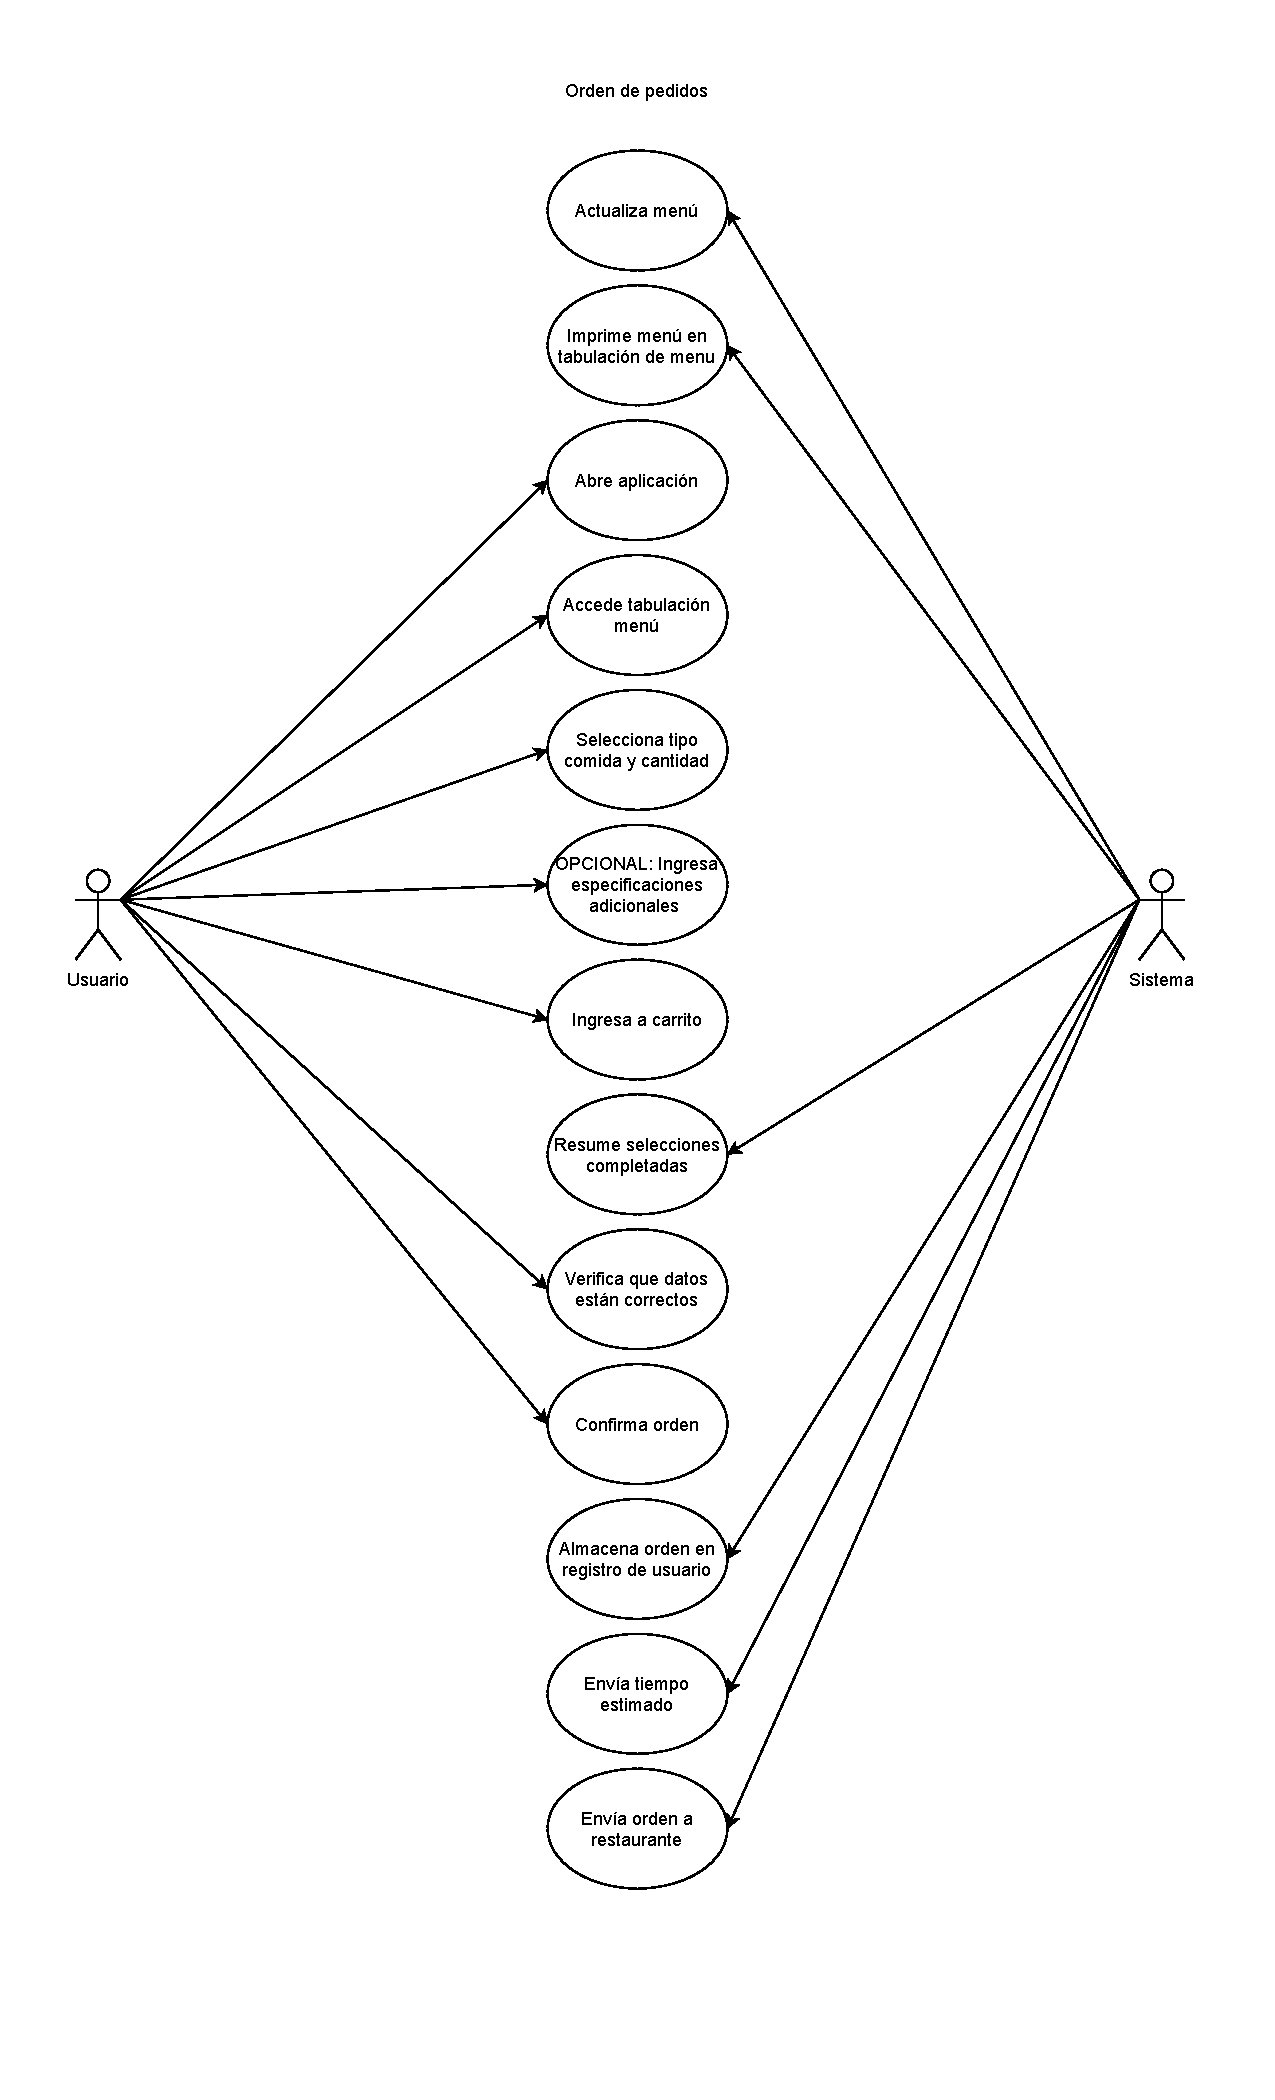
\includegraphics[scale=0.23]{imagenes/DCU Orden de Pedidos1.pdf}
\caption{ Orden de Pedidos}
\end{figure}


\begin{figure}[H]
\centering
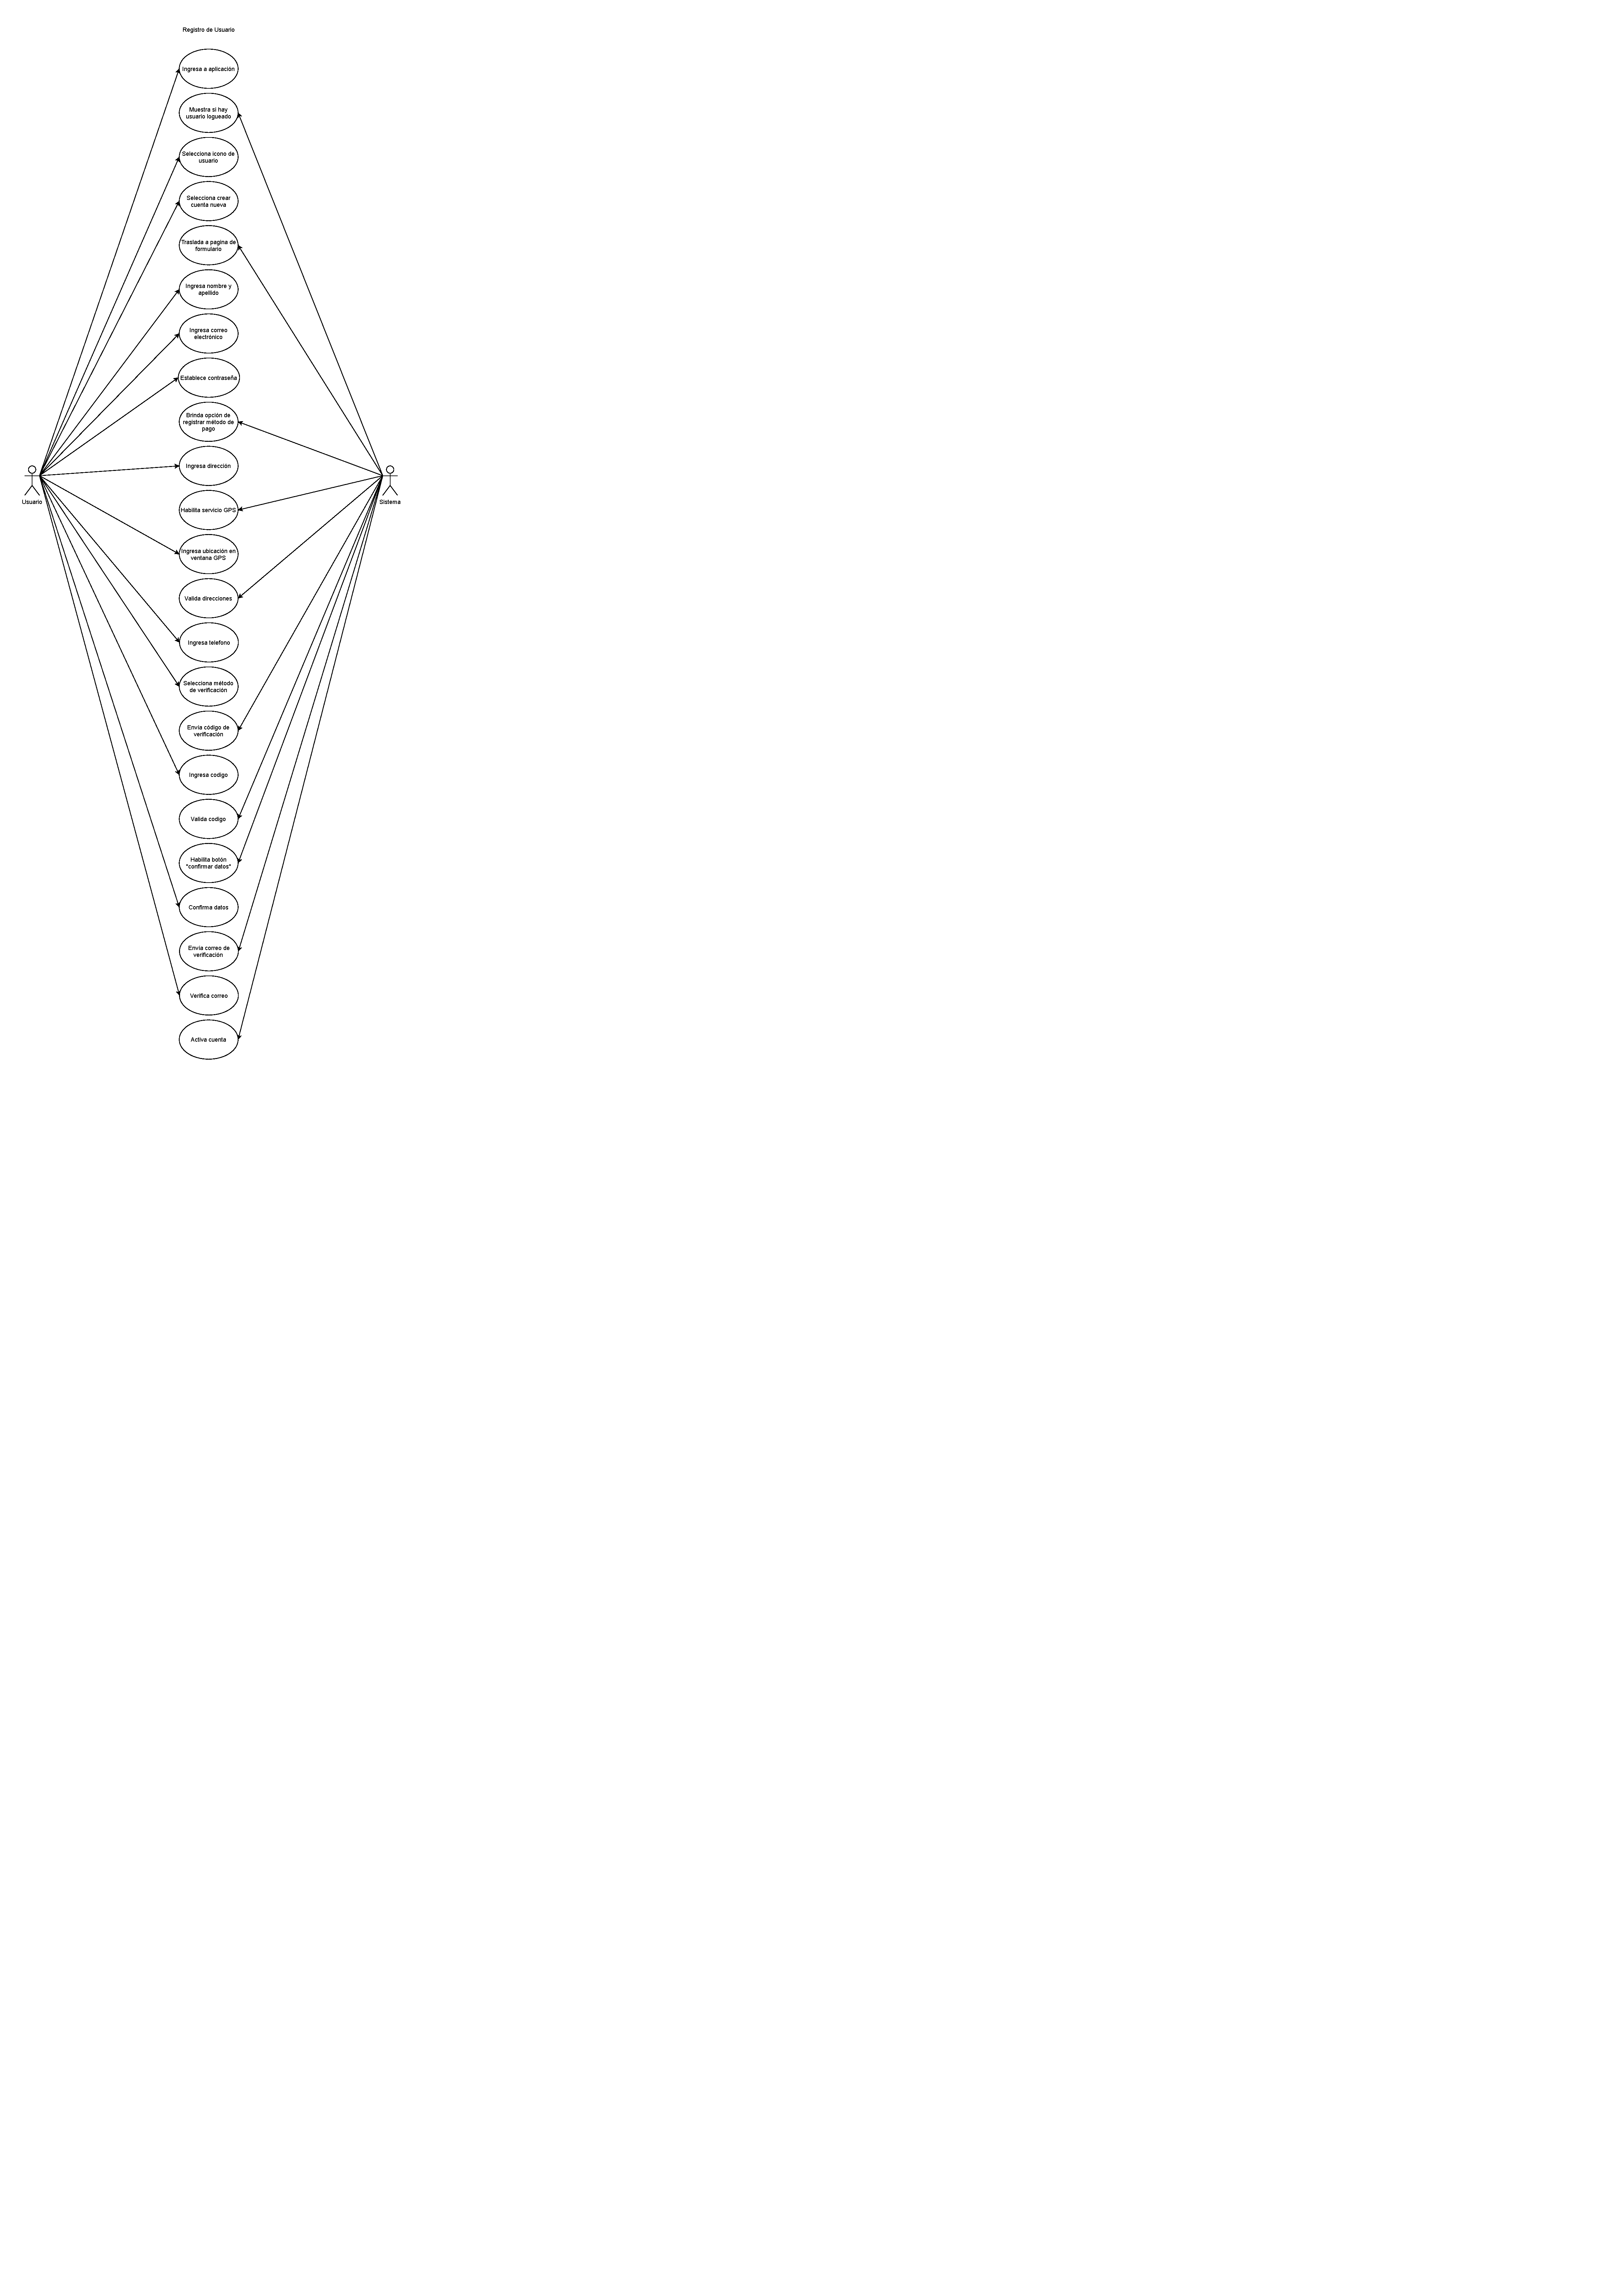
\includegraphics[scale=0.19]{imagenes/DCU Registro de Usuario2.pdf}
\caption{ Registro de Usuario}
\end{figure}


\begin{figure}[H]
\centering
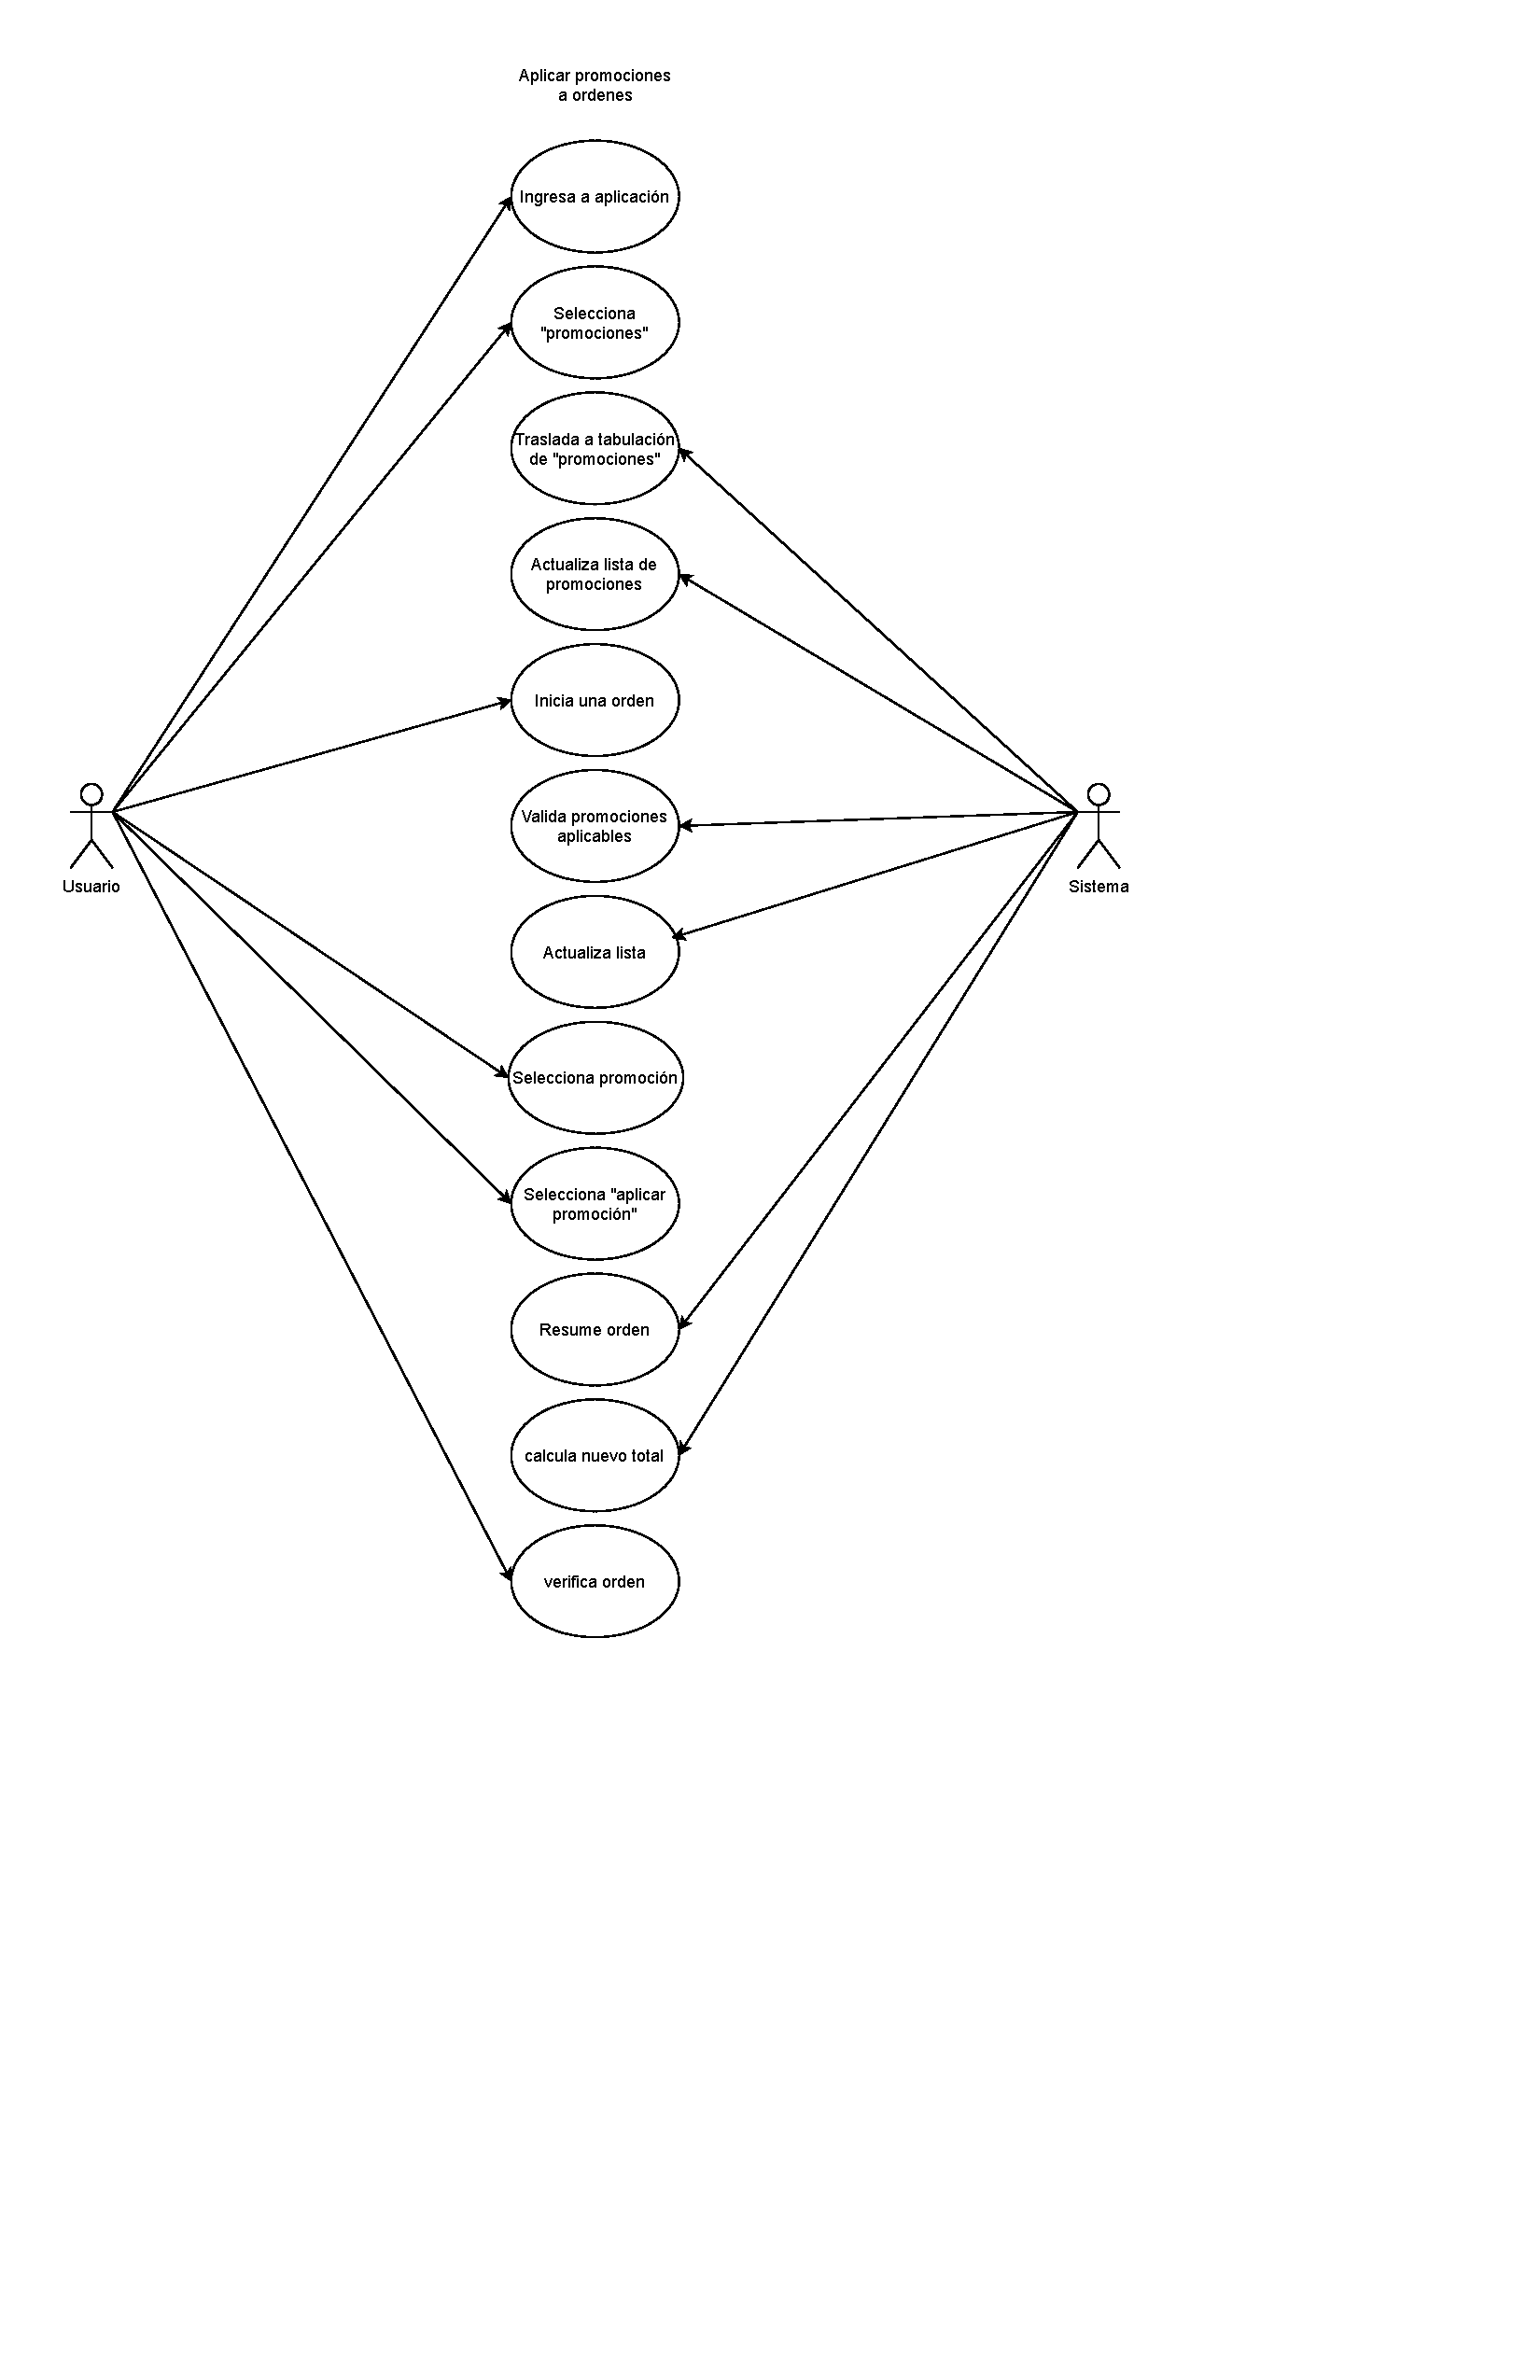
\includegraphics[scale=0.24]{imagenes/DCU Aplicar promociones a ordenes3.pdf}
\caption{Aplicar promociones a ordenes}
\end{figure}

\begin{figure}[H]
\centering
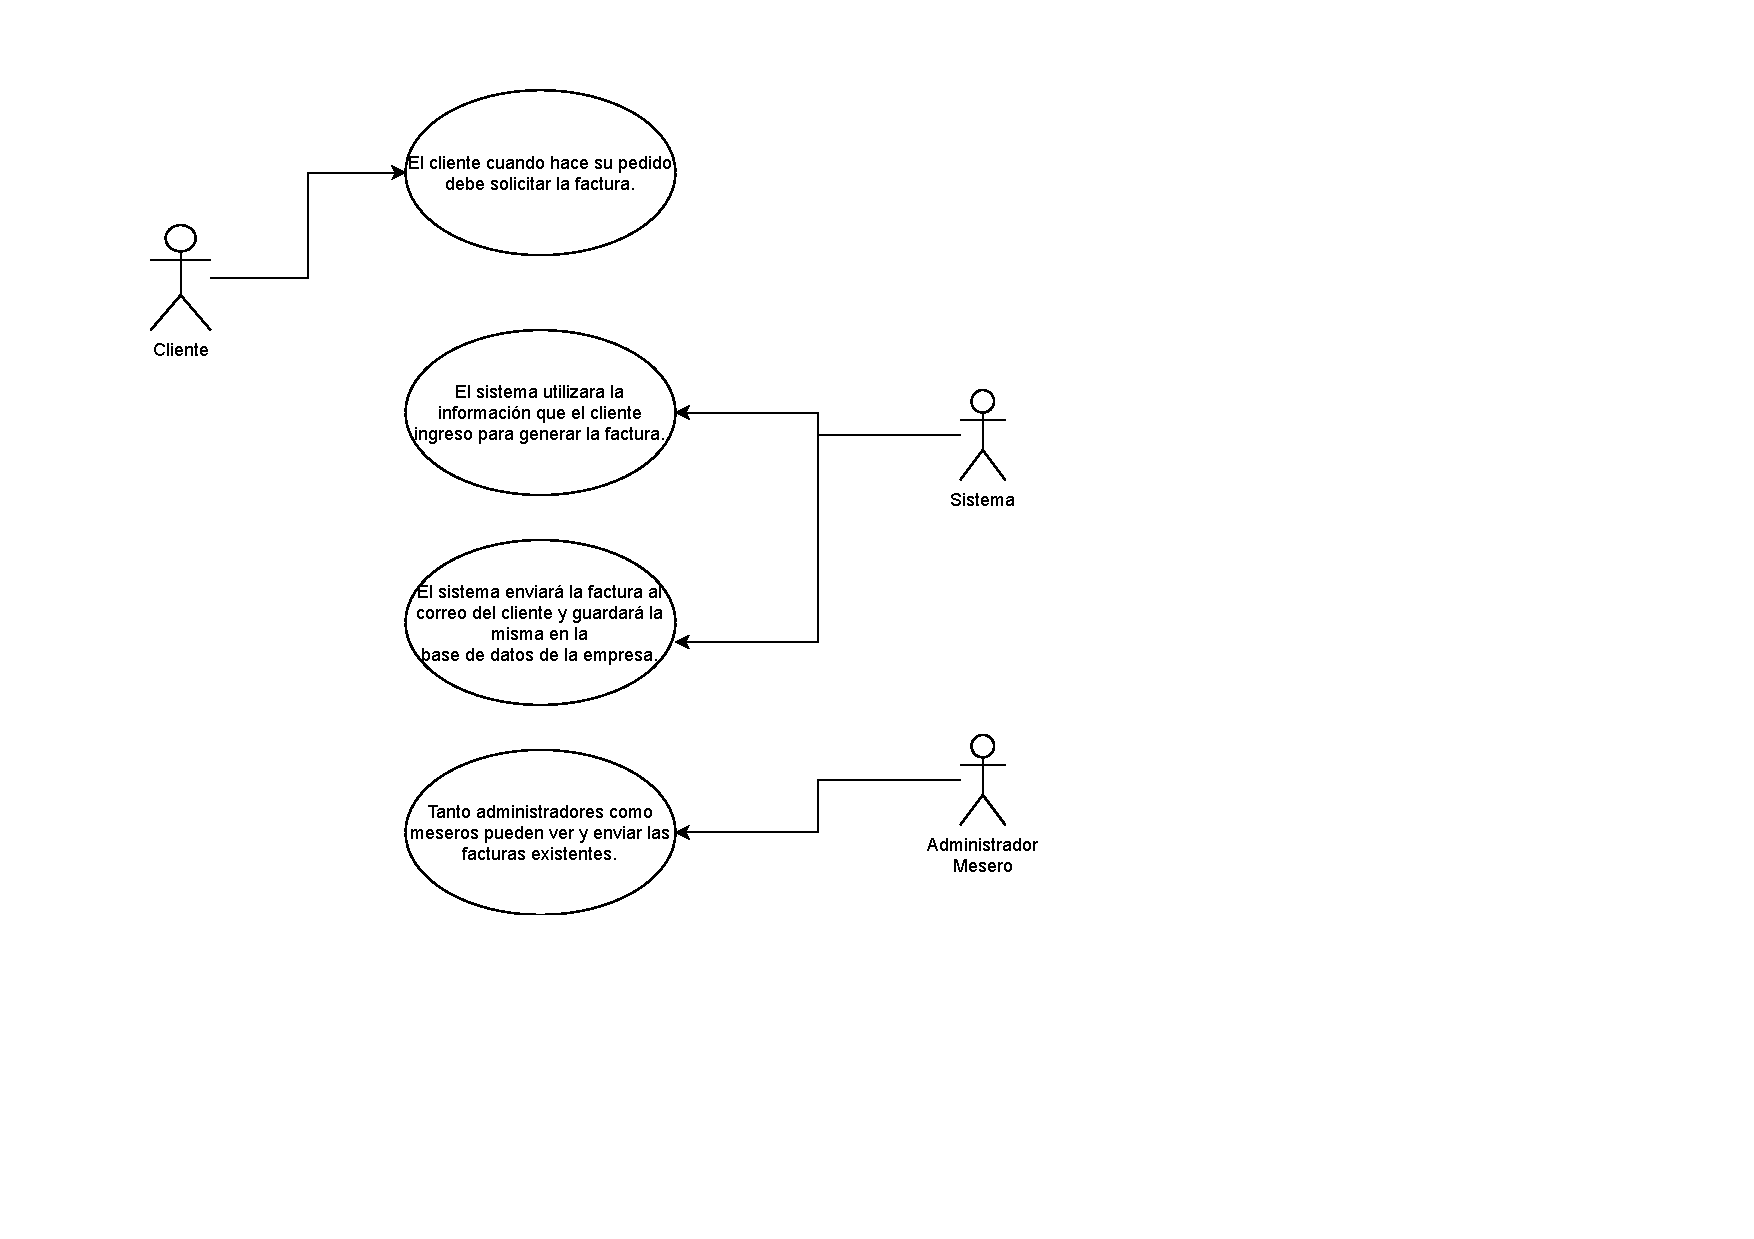
\includegraphics[scale=0.24]{imagenes/Diagrama_requerimiento4 (1).pdf}
\caption{Facturación Instantanea}
\end{figure}

\begin{figure}[H]
\centering
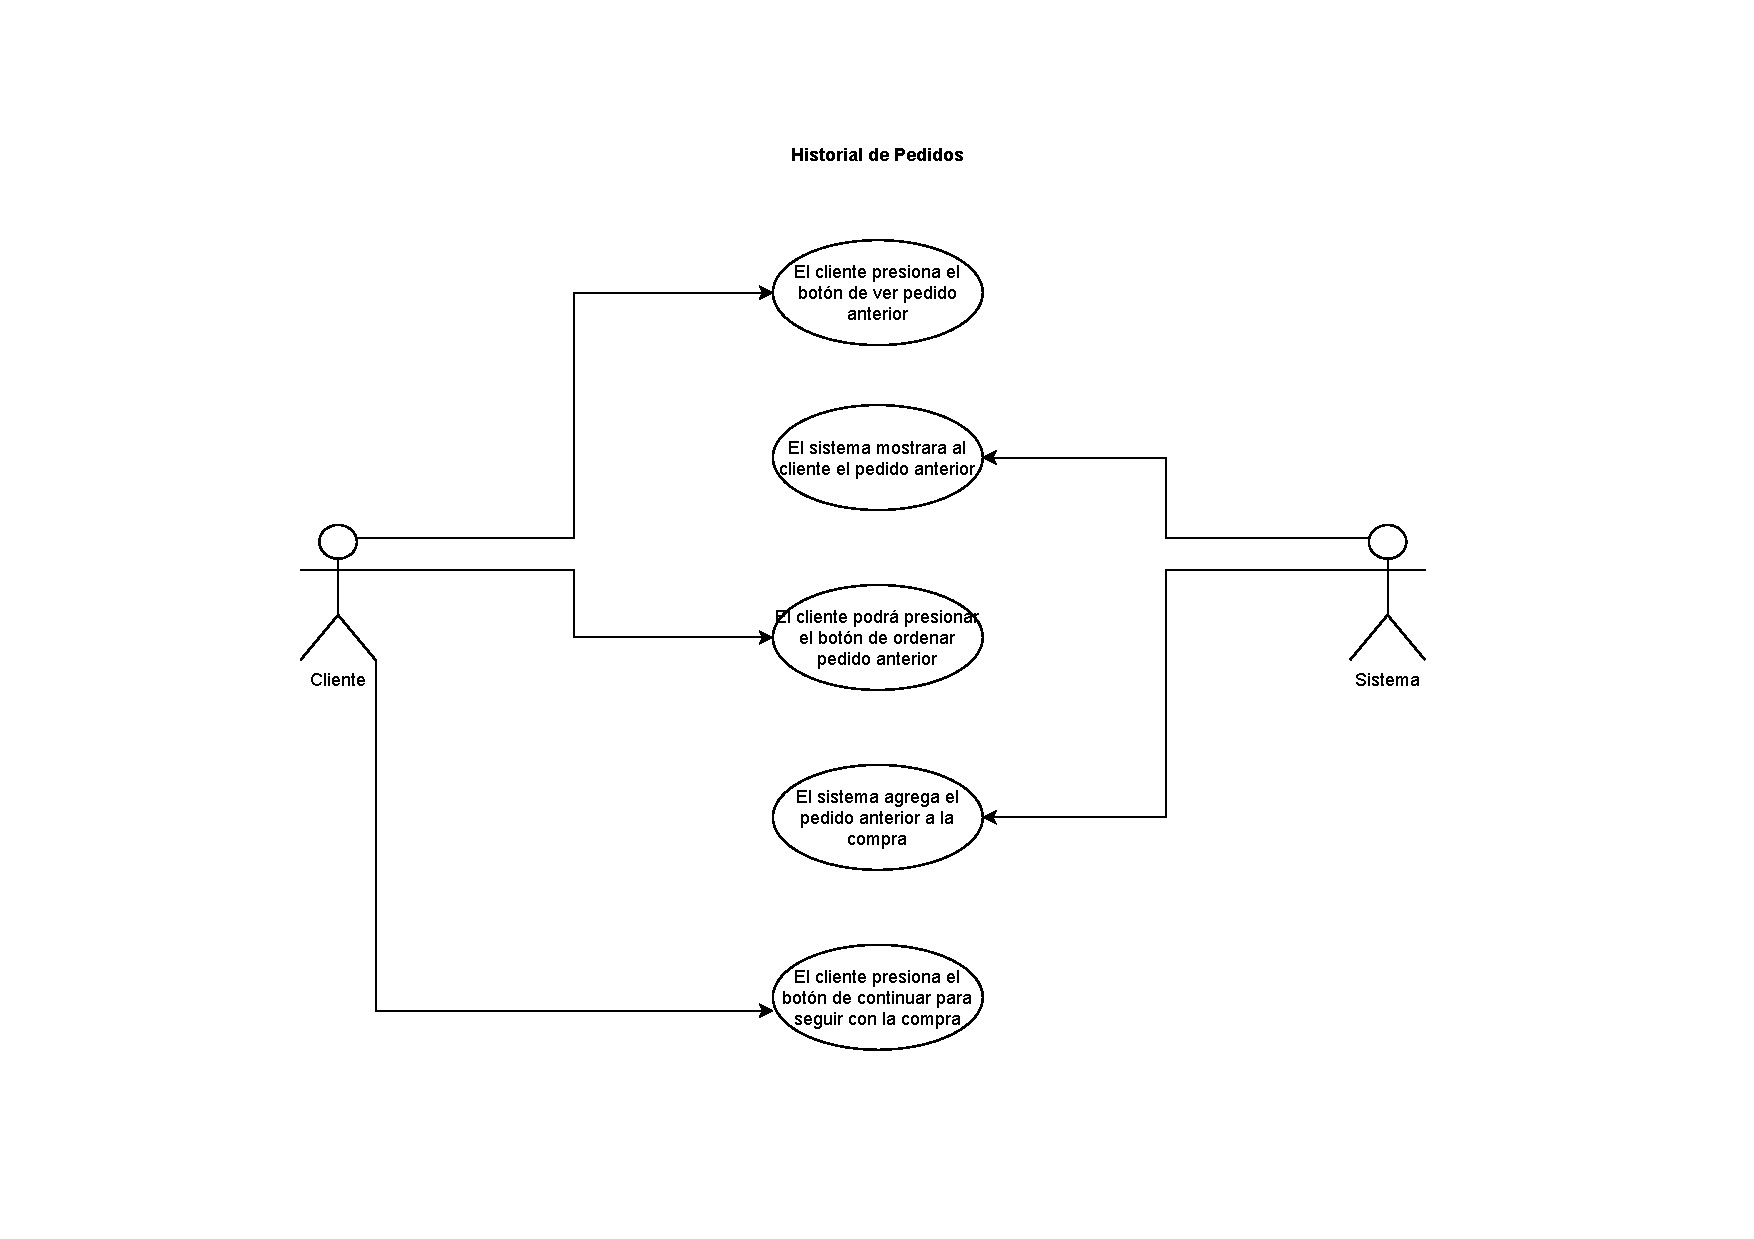
\includegraphics[scale=0.24]{imagenes/Caso de uso 5.pdf}
\caption{Historial de pedido}
\end{figure}

\begin{figure}[H]
\centering
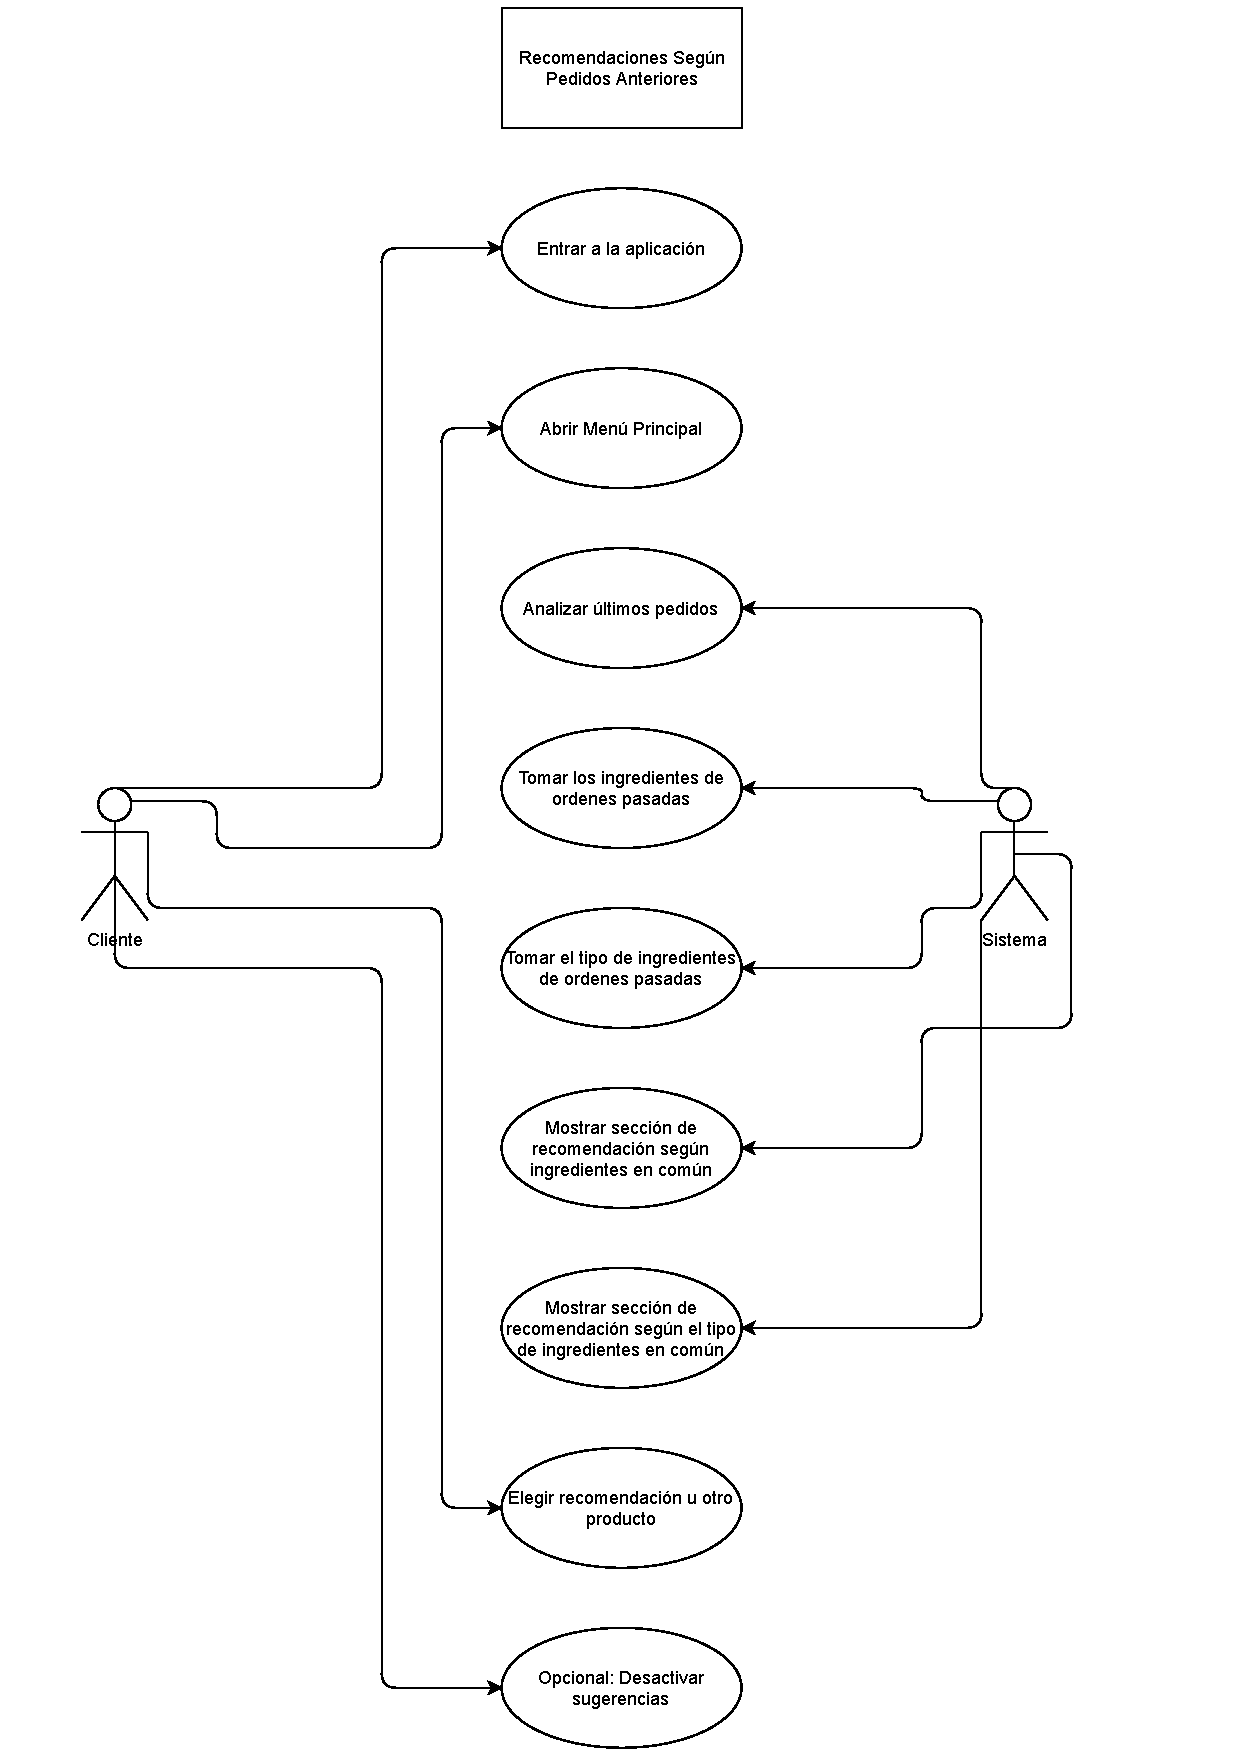
\includegraphics[scale=0.24]{imagenes/Requerimiento 6 (1).pdf}
\caption{Mostrar Recomendaciones Según Pedidos Anteriores}
\end{figure}

\begin{figure}[H]
\centering
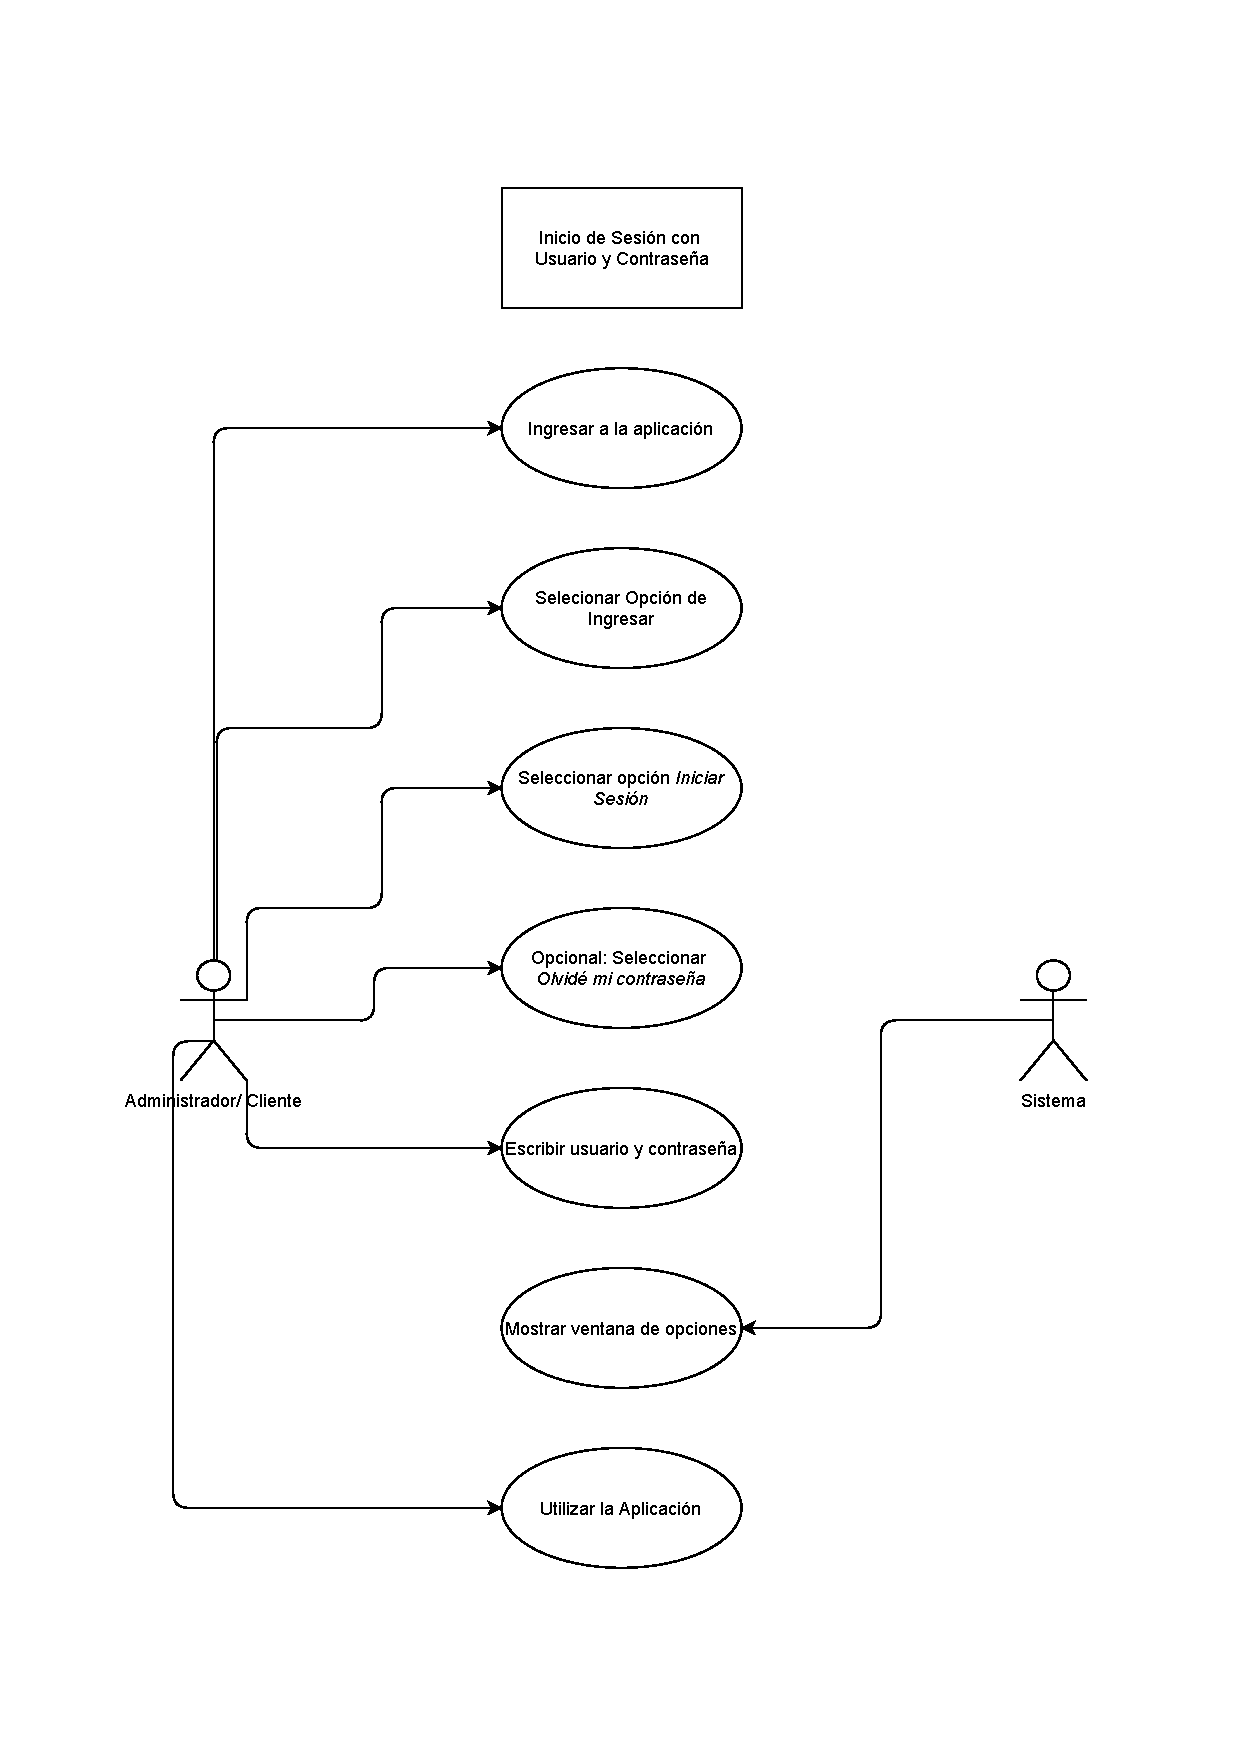
\includegraphics[scale=0.24]{imagenes/Requerimiento 7 (1).pdf}
\caption{Inicio de Sesión con Usuario y Contraseña}
\end{figure}

\begin{figure}[H]
\centering
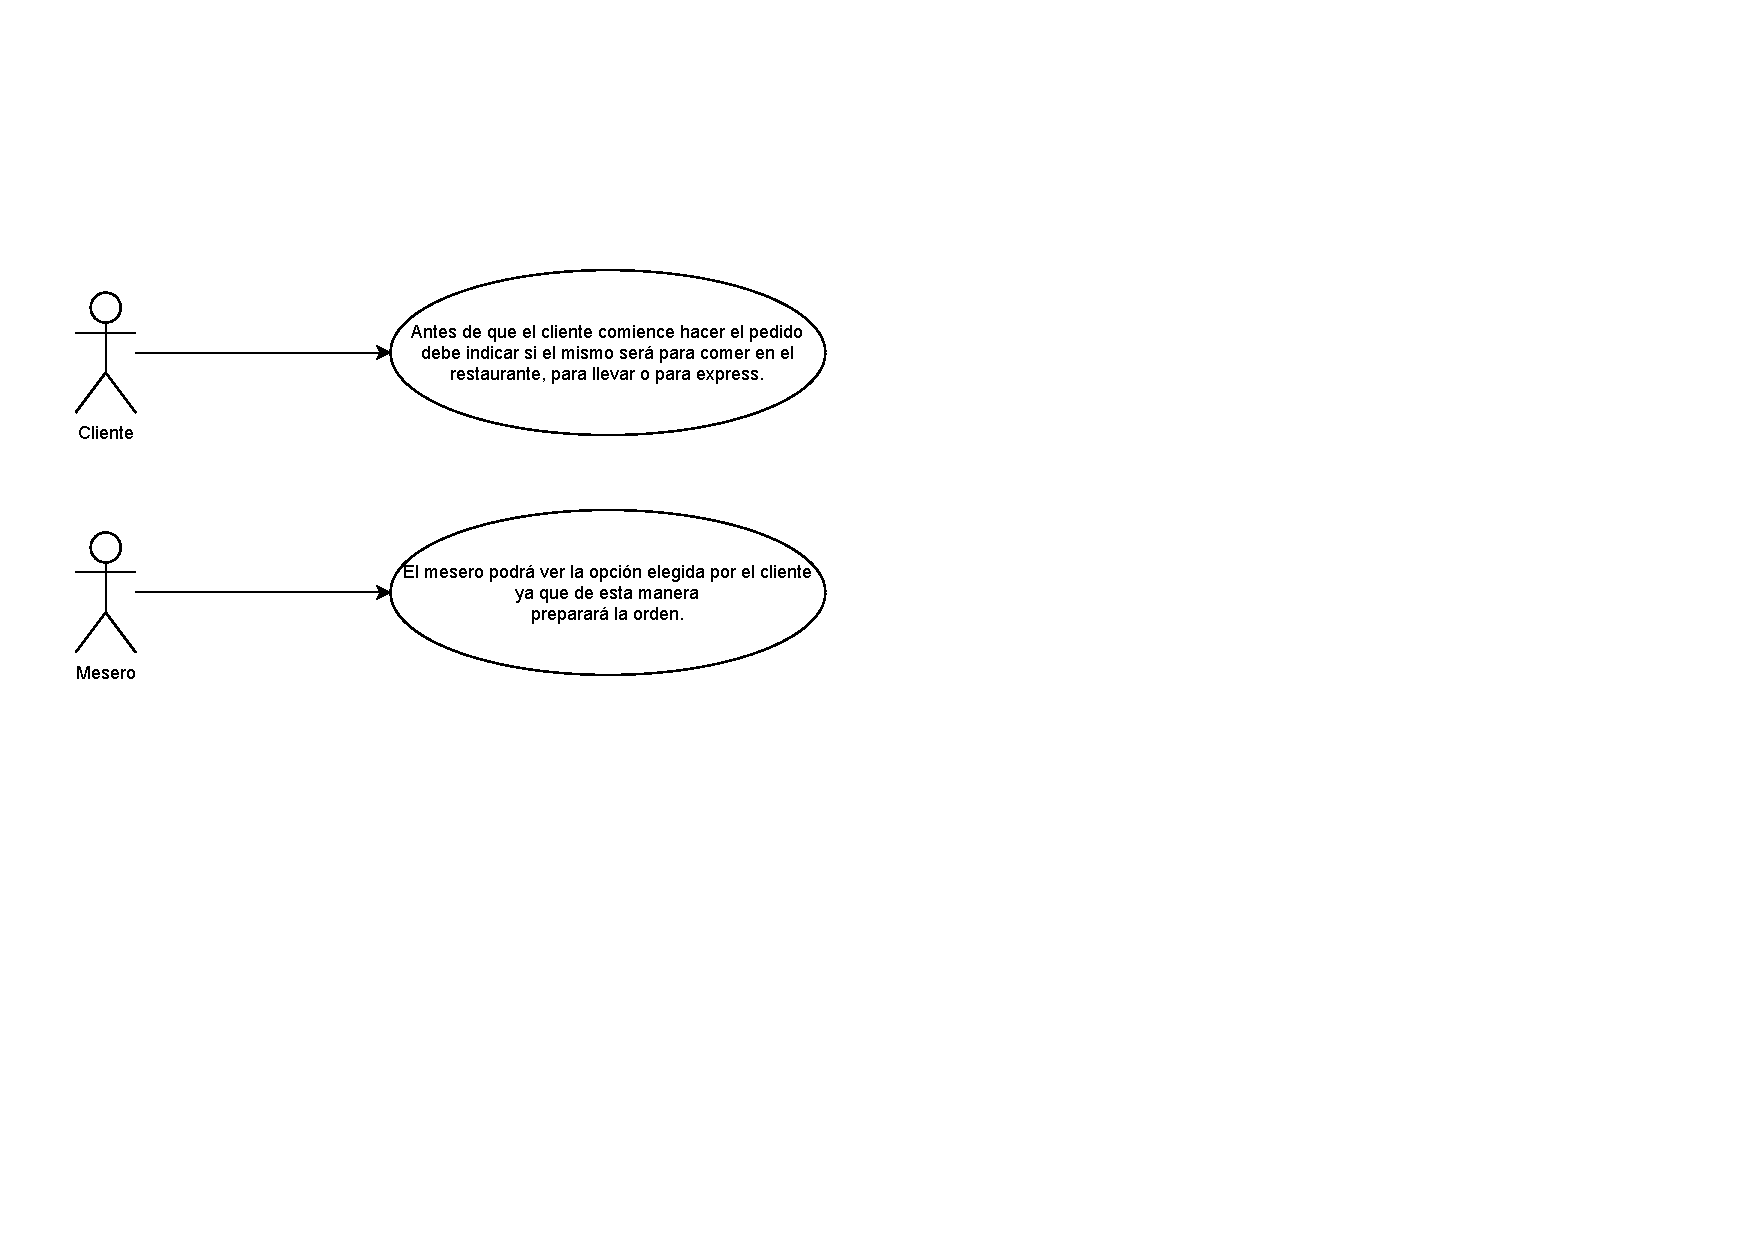
\includegraphics[scale=0.24]{imagenes/Diagrama_requerimiento8.pdf}
\caption{Tipo de servicio (Express o restaurante}
\end{figure}

\begin{figure}[H]
\centering
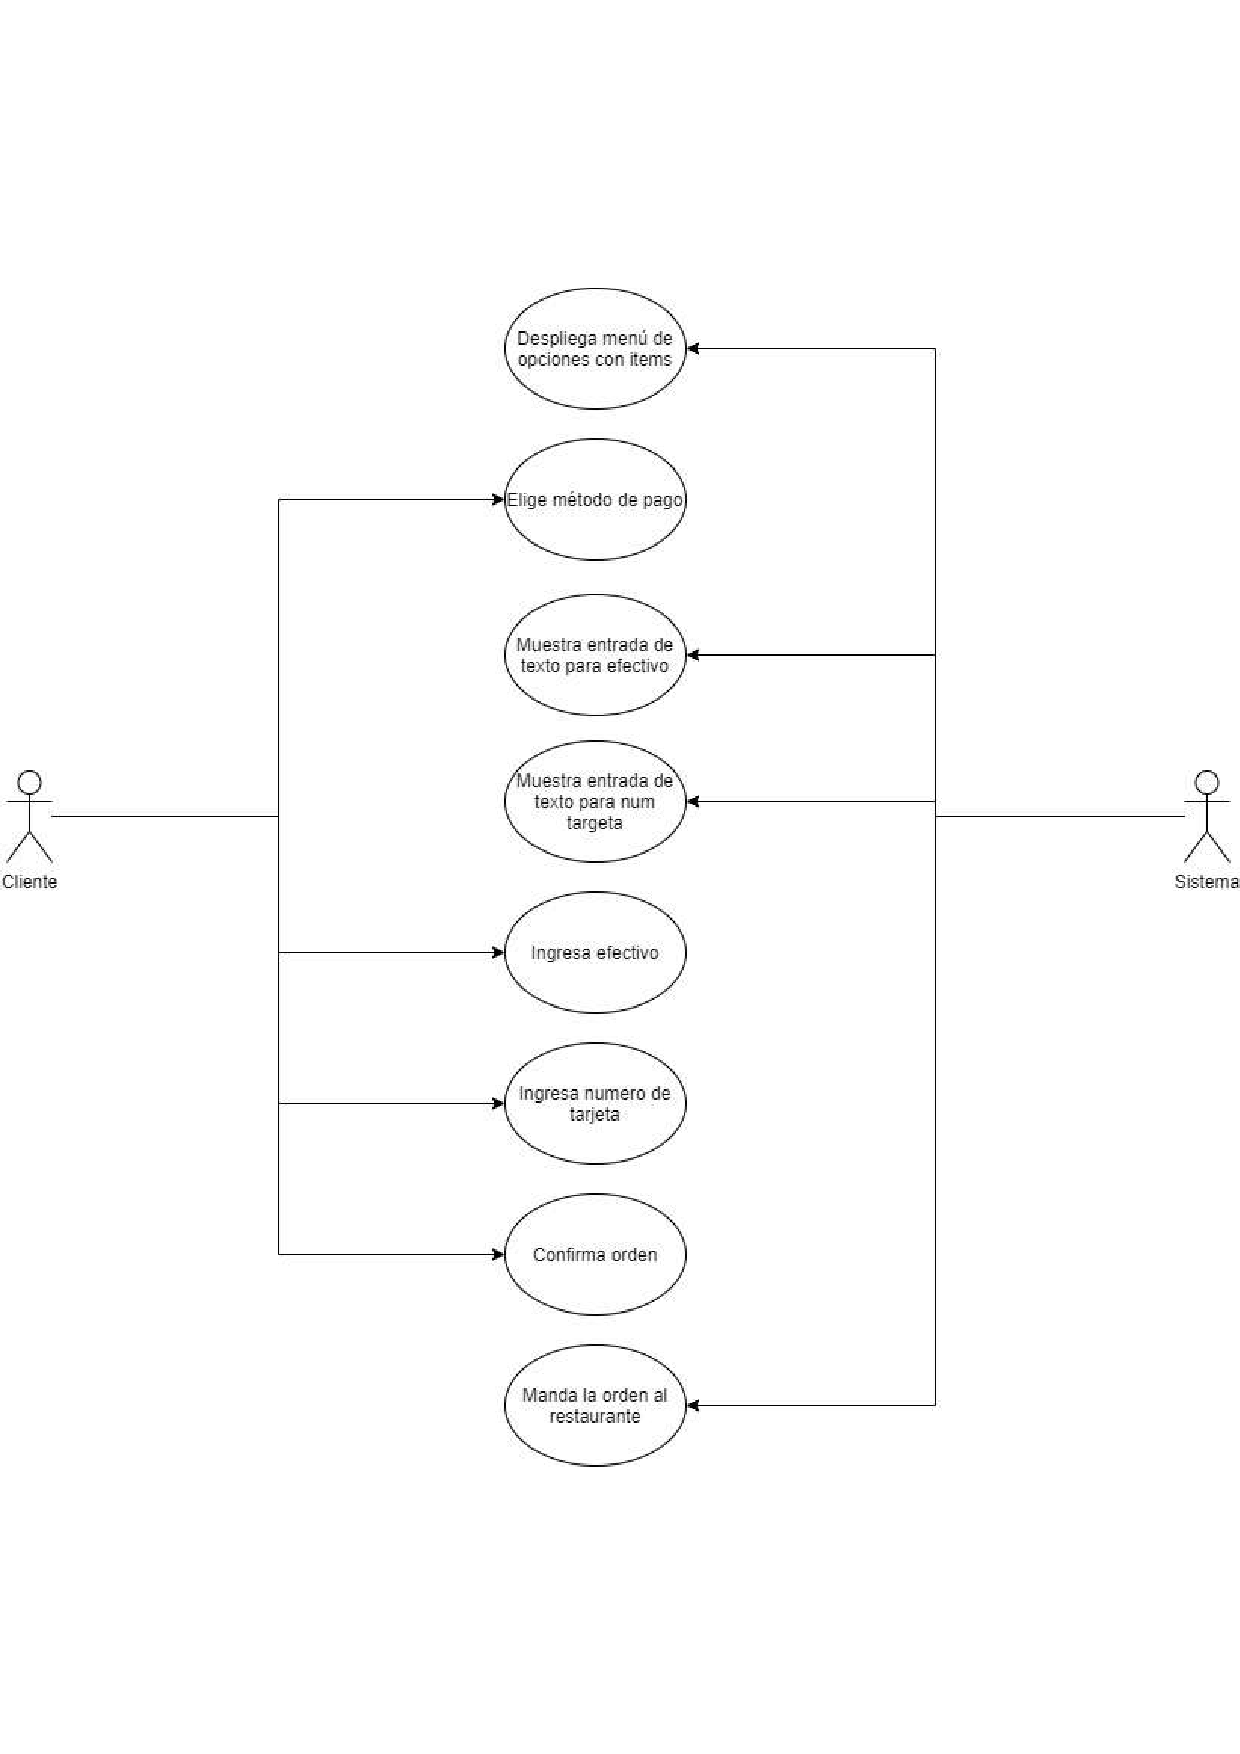
\includegraphics[scale=0.24]{imagenes/Requerimiento9.pdf}
\caption{Distintos Métodos de Pago}
\end{figure}


\begin{figure}[H]
\centering
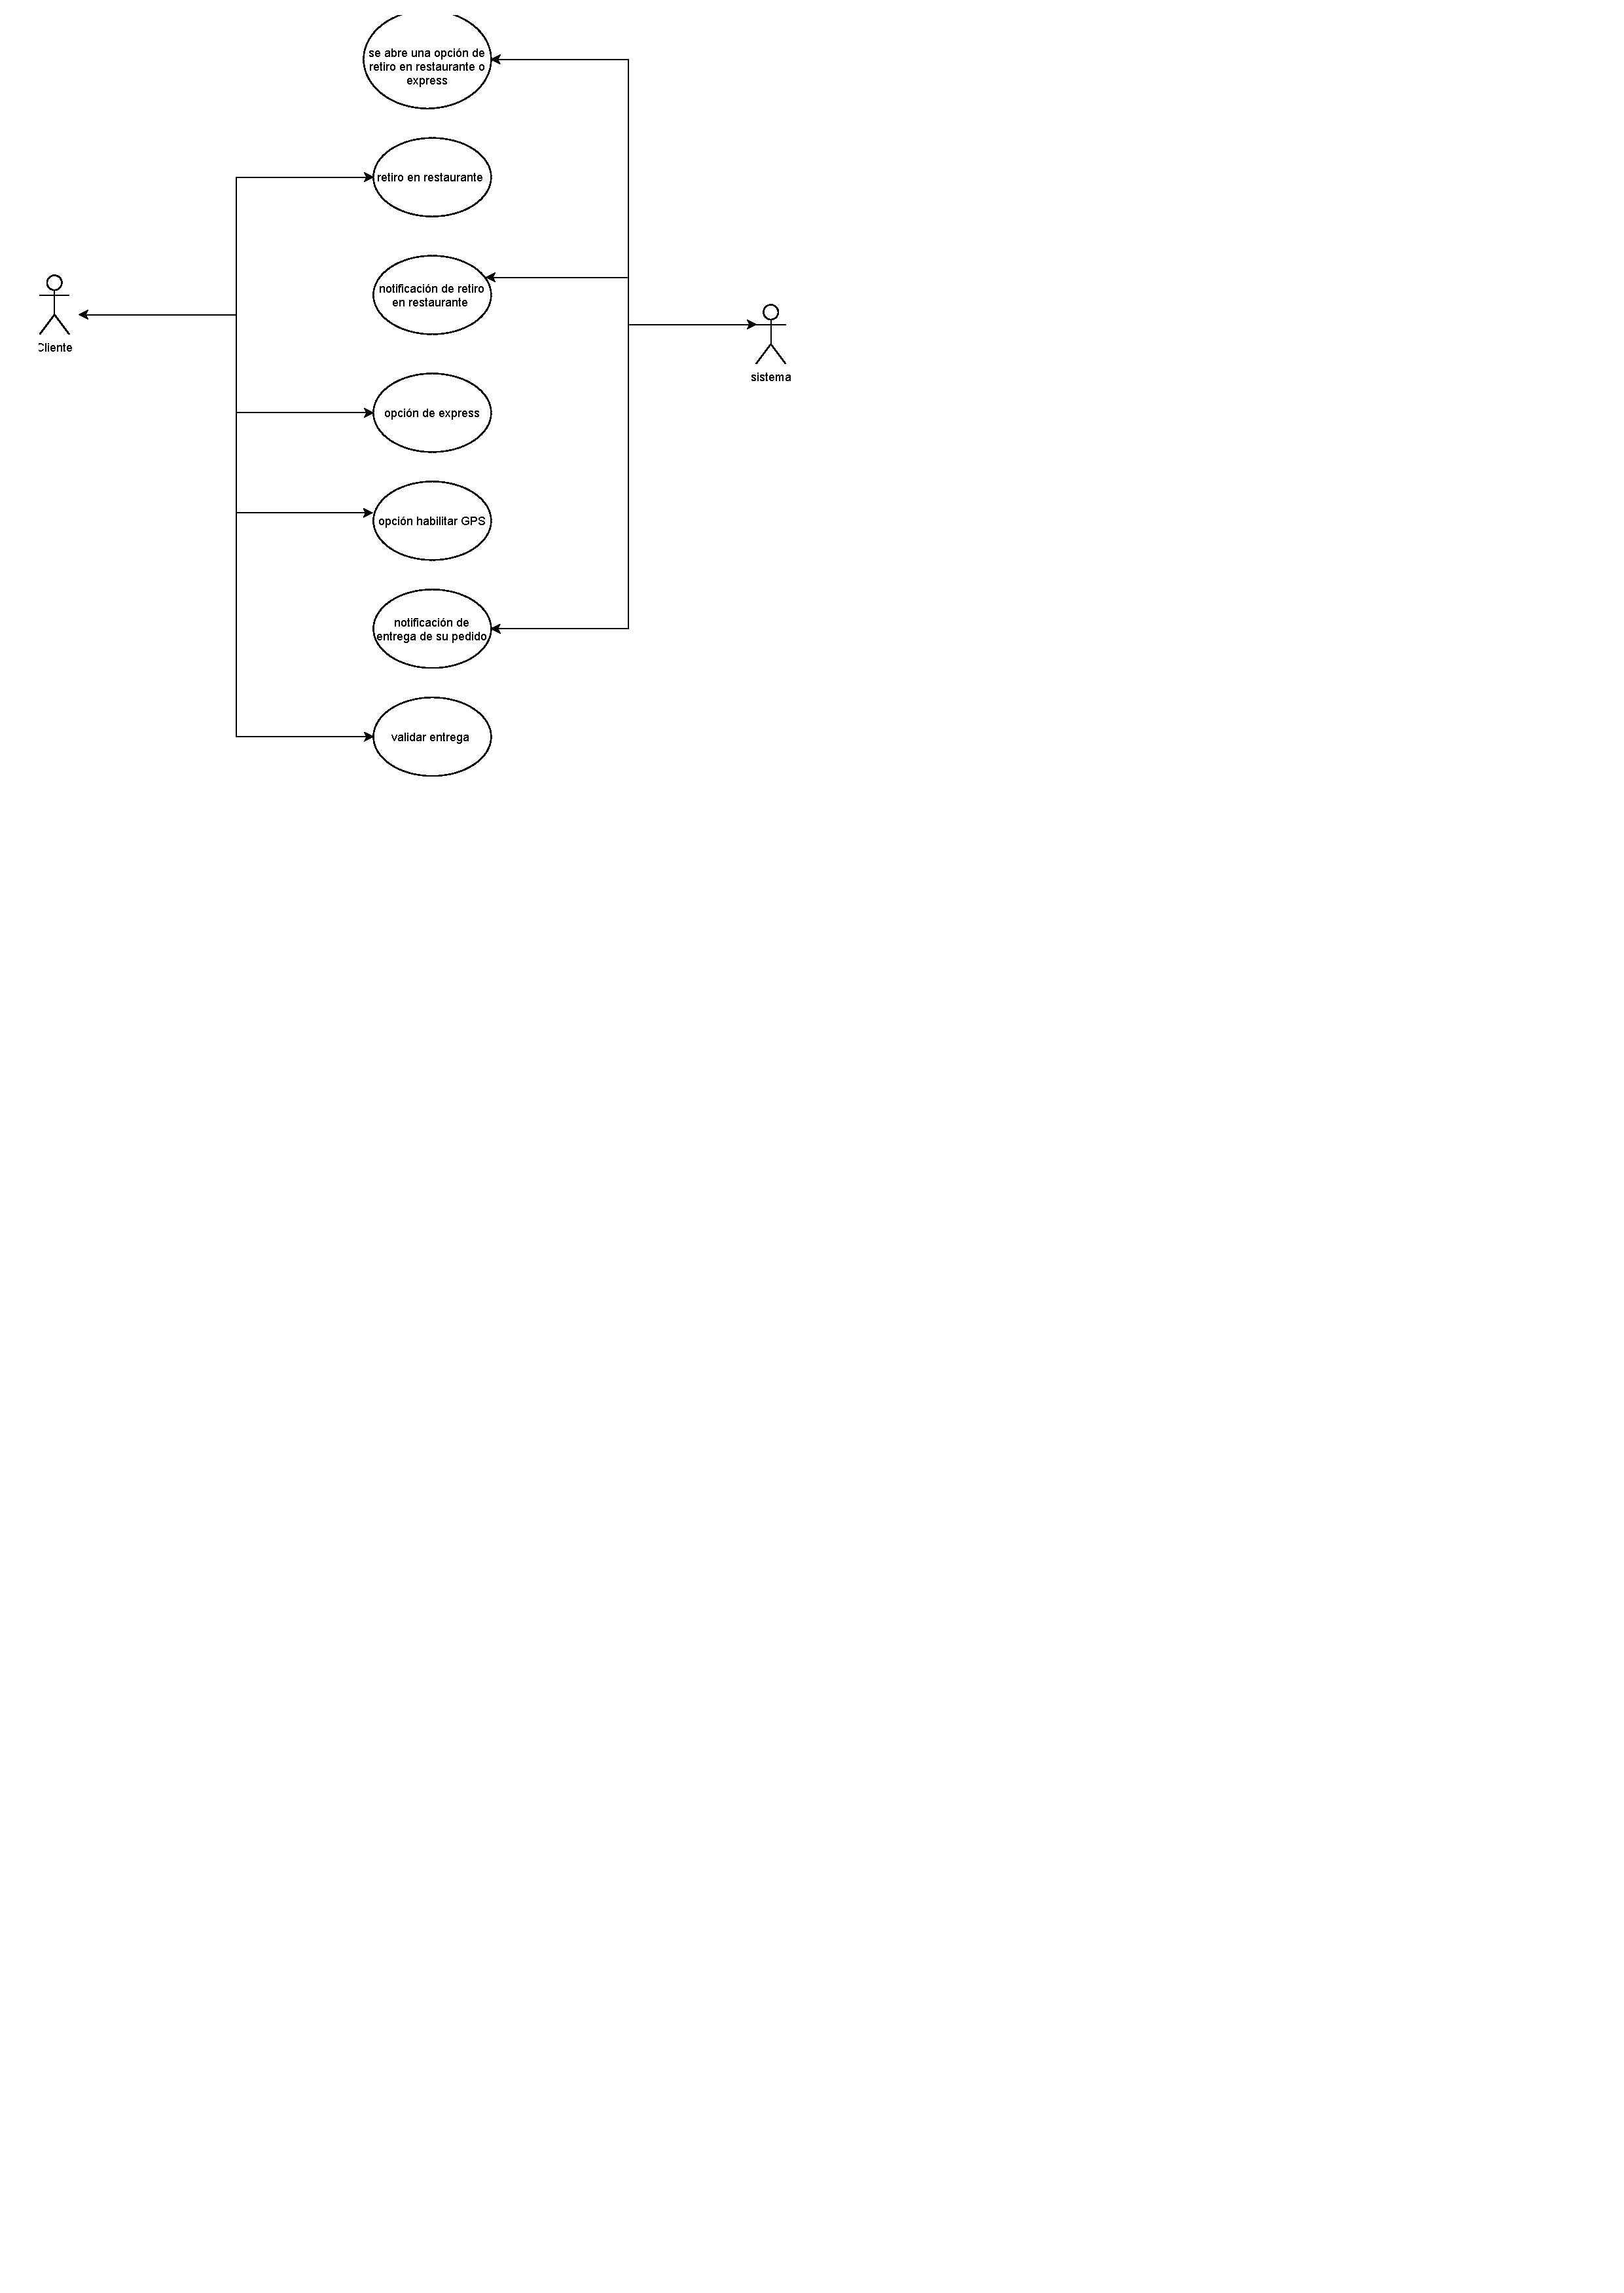
\includegraphics[scale=0.23]{imagenes/requerimiento .pdf}
\caption{Capacidad de habilitar la ubicación en tiempo real para mayor precision en los pedidos express}
\end{figure}



\end{document}